%==============================================================================
% tento soubor pouzijte jako zaklad
% this file should be used as a base for the thesis
% Autoři / Authors: 2008 Michal Bidlo, 2019 Jaroslav Dytrych
% Kontakt pro dotazy a připomínky: sablona@fit.vutbr.cz
% Contact for questions and comments: sablona@fit.vutbr.cz
%==============================================================================
% kodovani: UTF-8 (zmena prikazem iconv, recode nebo cstocs)
% encoding: UTF-8 (you can change it by command iconv, recode or cstocs)
%------------------------------------------------------------------------------
% zpracování / processing: make, make pdf, make clean
%==============================================================================
% Soubory, které je nutné upravit nebo smazat: / Files which have to be edited or deleted:
%   projekt-20-literatura-bibliography.bib - literatura / bibliography
%   projekt-01-kapitoly-chapters.tex - obsah práce / the thesis content
%   projekt-01-kapitoly-chapters-en.tex - obsah práce v angličtině / the thesis content in English
%   projekt-30-prilohy-appendices.tex - přílohy / appendices
%   projekt-30-prilohy-appendices-en.tex - přílohy v angličtině / appendices in English
%==============================================================================
\documentclass[zadani,slovak]{fitthesis} % bez zadání - pro začátek práce, aby nebyl problém s překladem
%\documentclass[english]{fitthesis} % without assignment - for the work start to avoid compilation problem
%\documentclass[zadani]{fitthesis} % odevzdani do wisu a/nebo tisk s barevnými odkazy - odkazy jsou barevné
%\documentclass[english,zadani]{fitthesis} % for submission to the IS FIT and/or print with color links - links are color
%\documentclass[zadani,print]{fitthesis} % pro černobílý tisk - odkazy jsou černé
%\documentclass[english,zadani,print]{fitthesis} % for the black and white print - links are black
%\documentclass[zadani,cprint]{fitthesis} % pro barevný tisk - odkazy jsou černé, znak VUT barevný
%\documentclass[english,zadani,cprint]{fitthesis} % for the print - links are black, logo is color
% * Je-li práce psaná v anglickém jazyce, je zapotřebí u třídy použít 
%   parametr english následovně:
%   If thesis is written in English, it is necessary to use 
%   parameter english as follows:
%      \documentclass[english]{fitthesis}
% * Je-li práce psaná ve slovenském jazyce, je zapotřebí u třídy použít 
%   parametr slovak následovně:
%   If the work is written in the Slovak language, it is necessary 
%   to use parameter slovak as follows:
%      \documentclass[slovak]{fitthesis}
% * Je-li práce psaná v anglickém jazyce se slovenským abstraktem apod., 
%   je zapotřebí u třídy použít parametry english a enslovak následovně:
%   If the work is written in English with the Slovak abstract, etc., 
%   it is necessary to use parameters english and enslovak as follows:
%      \documentclass[english,enslovak]{fitthesis}

% Základní balíčky jsou dole v souboru šablony fitthesis.cls
% Basic packages are at the bottom of template file fitthesis.cls
% zde můžeme vložit vlastní balíčky / you can place own packages here

% Kompilace po částech (rychlejší, ale v náhledu nemusí být vše aktuální)
% Compilation piecewise (faster, but not all parts in preview will be up-to-date)
% \usepackage{subfiles}

% Nastavení cesty k obrázkům
% Setting of a path to the pictures
%\graphicspath{{obrazky-figures/}{./obrazky-figures/}}
%\graphicspath{{obrazky-figures/}{../obrazky-figures/}}

%---rm---------------
\renewcommand{\rmdefault}{lmr}%zavede Latin Modern Roman jako rm / set Latin Modern Roman as rm
%---sf---------------
\renewcommand{\sfdefault}{qhv}%zavede TeX Gyre Heros jako sf
%---tt------------
\renewcommand{\ttdefault}{lmtt}% zavede Latin Modern tt jako tt

% vypne funkci šablony, která automaticky nahrazuje uvozovky,
% aby nebyly prováděny nevhodné náhrady v popisech API apod.
% disables function of the template which replaces quotation marks
% to avoid unnecessary replacements in the API descriptions etc.
\csdoublequotesoff



\usepackage{url}


% =======================================================================
% balíček "hyperref" vytváří klikací odkazy v pdf, pokud tedy použijeme pdflatex
% problém je, že balíček hyperref musí být uveden jako poslední, takže nemůže
% být v šabloně
% "hyperref" package create clickable links in pdf if you are using pdflatex.
% Problem is that this package have to be introduced as the last one so it 
% can not be placed in the template file.
\ifWis
\ifx\pdfoutput\undefined % nejedeme pod pdflatexem / we are not using pdflatex
\else
  \usepackage{color}
  \usepackage[unicode,colorlinks,hyperindex,plainpages=false,pdftex]{hyperref}
  \definecolor{hrcolor-ref}{RGB}{223,52,30}
  \definecolor{hrcolor-cite}{HTML}{2F8F00}
  \definecolor{hrcolor-urls}{HTML}{092EAB}
  \hypersetup{
	linkcolor=hrcolor-ref,
	citecolor=hrcolor-cite,
	filecolor=magenta,
	urlcolor=hrcolor-urls
  }
  \def\pdfBorderAttrs{/Border [0 0 0] }  % bez okrajů kolem odkazů / without margins around links
  \pdfcompresslevel=9
\fi
\else % pro tisk budou odkazy, na které se dá klikat, černé / for the print clickable links will be black
\ifx\pdfoutput\undefined % nejedeme pod pdflatexem / we are not using pdflatex
\else
  \usepackage{color}
  \usepackage[unicode,colorlinks,hyperindex,plainpages=false,pdftex,urlcolor=black,linkcolor=black,citecolor=black]{hyperref}
  \definecolor{links}{rgb}{0,0,0}
  \definecolor{anchors}{rgb}{0,0,0}
  \def\AnchorColor{anchors}
  \def\LinkColor{links}
  \def\pdfBorderAttrs{/Border [0 0 0] } % bez okrajů kolem odkazů / without margins around links
  \pdfcompresslevel=9
\fi
\fi
% Řešení problému, kdy klikací odkazy na obrázky vedou za obrázek
% This solves the problems with links which leads after the picture
\usepackage[all]{hypcap}

% Informace o práci/projektu / Information about the thesis
%---------------------------------------------------------------------------
\projectinfo{
  %Prace / Thesis
  project={BP},            %typ práce BP/SP/DP/DR  / thesis type (SP = term project)
  year={2021},             % rok odevzdání / year of submission
  date=\today,             % datum odevzdání / submission date
  %Nazev prace / thesis title
  title.cs={Webový editor prezentací},  % název práce v češtině či slovenštině (dle zadání) / thesis title in czech language (according to assignment)
  title.en={Presentations Web Editor}, % název práce v angličtině / thesis title in english
  %title.length={14.5cm}, % nastavení délky bloku s titulkem pro úpravu zalomení řádku (lze definovat zde nebo níže) / setting the length of a block with a thesis title for adjusting a line break (can be defined here or below)
  %sectitle.length={14.5cm}, % nastavení délky bloku s druhým titulkem pro úpravu zalomení řádku (lze definovat zde nebo níže) / setting the length of a block with a second thesis title for adjusting a line break (can be defined here or below)
  %Autor / Author
  author.name={Adam},   % jméno autora / author name
  author.surname={Abrahám},   % příjmení autora / author surname 
  %author.title.p={Bc.}, % titul před jménem (nepovinné) / title before the name (optional)
  %author.title.a={Ph.D.}, % titul za jménem (nepovinné) / title after the name (optional)
  %Ustav / Department
  department={UIFS}, % doplňte příslušnou zkratku dle ústavu na zadání: UPSY/UIFS/UITS/UPGM / fill in appropriate abbreviation of the department according to assignment: UPSY/UIFS/UITS/UPGM
  % Školitel / supervisor
  supervisor.name={Radek},   % jméno školitele / supervisor name 
  supervisor.surname={Burget},   % příjmení školitele / supervisor surname
  supervisor.title.p={Ing.},   %titul před jménem (nepovinné) / title before the name (optional)
  supervisor.title.a={Ph.D.},    %titul za jménem (nepovinné) / title after the name (optional)
  % Klíčová slova / keywords
  keywords.cs={Webová aplikácia, Editor, Prezentácia, Markdown, JavaScript, TypeScript, NoSQL, MongoDB, Node.js, Express.js, REST, Vue.js, Nuxt.js, Buefy, Reveal.js, Cypress}, % klíčová slova v českém či slovenském jazyce / keywords in czech or slovak language
  keywords.en={Web application, Editor, Presentation, Markdown, JavaScript, TypeScript, NoSQL, MongoDB, Node.js, Express.js, REST, Vue.js, Nuxt.js, Buefy, Reveal.js, Cypress}, % klíčová slova v anglickém jazyce / keywords in english
  %keywords.en={Here, individual keywords separated by commas will be written in English.},
  % Abstrakt / Abstract
  abstract.cs={Cieľom tejto práce je implementácia webovej aplikácie s tlstým klientom pre spravovanie prezentácií s obsahom typu Markdown, ktorý sa následne prezentuje pomocou frameworku Reveal.js. Frontend aplikácie je vytvorený pomocou Vue.js, backend pomocou Express.js a ako úložisko údajov som si zvolil MongoDB, NoSQL dokumentovú databázu. Frontend a backend časti aplikácie komunikujú medzi sebou cez technológiu REST. Výsledná aplikácia umožňuje užívateľom zobrazovať, upravovať a vytvárať viacero verzií danej prezentácie.  Práca naďalej obsahuje popis, porovnanie súčasných technológií a zdôvodnenie ich výberu. }, % abstrakt v českém či slovenském jazyce / abstract in czech or slovak language
  abstract.en={ The aim of this thesis is to implement a web application to manage presentations with Markdown content, which is then presented through Reveal.js framework . Frontend of the application is created with Vue.js, backend with Express.js and for data storage I have chosen MongoDB, a NoSQL document database. Frontend and backend parts of the application communicate with each other through REST technology. The application allows users to view, edit and create more versions of the same presentation. This thesis furthermore contains description, comparison of current technologies and substantiation of their selection. }, % abstrakt v anglickém jazyce / abstract in english
  %abstract.en={An abstract of the work in English will be written in this paragraph.},
  % Prohlášení (u anglicky psané práce anglicky, u slovensky psané práce slovensky) / Declaration (for thesis in english should be in english)
  declaration={Prohlašuji, že jsem tuto bakalářskou práci vypracoval samostatně pod vedením pana profesora Radeka Burgeta.
Uvedl jsem všechny literární prameny, publikace a další zdroje, ze kterých jsem čerpal.},
  %declaration={I hereby declare that this Bachelor's thesis was prepared as an original work by the author under the supervision of Mr. X
% The supplementary information was provided by Mr. Y
% I have listed all the literary sources, publications and other sources, which were used during the preparation of this thesis.},
  % Poděkování (nepovinné, nejlépe v jazyce práce) / Acknowledgement (optional, ideally in the language of the thesis)
  acknowledgment={Moje poďakovanie patrí vedúcemu práce, profesorovi Radekovi Burgetovi za jeho rady, doporučenia a za pomoc pri tvorbe tejto práce.},
  %acknowledgment={Here it is possible to express thanks to the supervisor and to the people which provided professional help
%(external submitter, consultant, etc.).},
  % Rozšířený abstrakt (cca 3 normostrany) - lze definovat zde nebo níže / Extended abstract (approximately 3 standard pages) - can be defined here or below
  %extendedabstract={Do tohoto odstavce bude zapsán rozšířený výtah (abstrakt) práce v českém (slovenském) jazyce.},
  %faculty={FIT}, % FIT/FEKT/FSI/FA/FCH/FP/FAST/FAVU/USI/DEF
  faculty.cs={Fakulta informačních technologií}, % Fakulta v češtině - pro využití této položky výše zvolte fakultu DEF / Faculty in Czech - for use of this entry select DEF above
  faculty.en={Faculty of Information Technology}, % Fakulta v angličtině - pro využití této položky výše zvolte fakultu DEF / Faculty in English - for use of this entry select DEF above
  department.cs={Ústav informačních systémů}, % Ústav v češtině - pro využití této položky výše zvolte ústav DEF nebo jej zakomentujte / Department in Czech - for use of this entry select DEF above or comment it out
  department.en={Department of Information Systems} % Ústav v angličtině - pro využití této položky výše zvolte ústav DEF nebo jej zakomentujte / Department in English - for use of this entry select DEF above or comment it out
}

% Rozšířený abstrakt (cca 3 normostrany) - lze definovat zde nebo výše / Extended abstract (approximately 3 standard pages) - can be defined here or above
%\extendedabstract{Do tohoto odstavce bude zapsán výtah (abstrakt) práce v českém (slovenském) jazyce.}

% nastavení délky bloku s titulkem pro úpravu zalomení řádku - lze definovat zde nebo výše / setting the length of a block with a thesis title for adjusting a line break - can be defined here or above
%\titlelength{14.5cm}
% nastavení délky bloku s druhým titulkem pro úpravu zalomení řádku - lze definovat zde nebo výše / setting the length of a block with a second thesis title for adjusting a line break - can be defined here or above
%\sectitlelength{14.5cm}

% řeší první/poslední řádek odstavce na předchozí/následující stránce
% solves first/last row of the paragraph on the previous/next page
\clubpenalty=10000
\widowpenalty=10000

% checklist
\newlist{checklist}{itemize}{1}
\setlist[checklist]{label=$\square$}

\begin{document}
  % Vysazeni titulnich stran / Typesetting of the title pages
  % ----------------------------------------------
  \maketitle
  % Obsah
  % ----------------------------------------------
  \setlength{\parskip}{0pt}

  {\hypersetup{hidelinks}\tableofcontents}
  
  % Seznam obrazku a tabulek (pokud prace obsahuje velke mnozstvi obrazku, tak se to hodi)
  % List of figures and list of tables (if the thesis contains a lot of pictures, it is good)
  \ifczech
    \renewcommand\listfigurename{Seznam obrázků}
  \fi
  \ifslovak
    \renewcommand\listfigurename{Zoznam obrázkov}
  \fi
  % {\hypersetup{hidelinks}\listoffigures}
  
  \ifczech
    \renewcommand\listtablename{Seznam tabulek}
  \fi
  \ifslovak
    \renewcommand\listtablename{Zoznam tabuliek}
  \fi
  % {\hypersetup{hidelinks}\listoftables}

  \ifODSAZ
    \setlength{\parskip}{0.5\bigskipamount}
  \else
    \setlength{\parskip}{0pt}
  \fi

  % vynechani stranky v oboustrannem rezimu
  % Skip the page in the two-sided mode
  \iftwoside
    \cleardoublepage
  \fi

  % Text prace / Thesis text
  % ----------------------------------------------
\chapter{Úvod}
Táto bakalárska práca sa zaoberá implementáciou webovej aplikácie pre správu prezentácií. Hlavnou výhodou oproti konkurenčným riešeniam je možnosť kopírovania snímok medzi prezentáciami a verzovania jednotlivých prezentácií. Týmto spôsobom sa vyhneme zbytočnému ukladaniu našej práce pod názvy \texttt{xy-final}, \texttt{xy-final-final} a podobne, s ktorými sme sa už určite viacerí stretli, a máme všetky naše predošlé verzie práce dostupné na jednom mieste . Cieľom aplikácie je umožniť užívateľom vytvárať a spravovať prezentácie pomocou značkovacieho jazyka Markdown.

TODO Kapitoly...


\chapter{Popis a porovnanie súčasných webových technológií}
\label{kapitola2}
Cieľom tejto kapitoly je informovať čitateľa o súčasných webových technológiách. Kapitola obsahuje krátky popis jednotlivých jazykov a technológií a ich porovnanie. Záver popisuje najpopulárnejšie pomocné webové rámce (ďalej označované ako \texttt{frameworky}) pre vytváranie prezentácií vo webovom prehliadači.

\section{Databáza}
Databáza\cite{database} je množina štrukturovaných údajov ktorá slúži na uloženie informácií. Tieto informácie si môže počítačový program, alebo človek pomocou dopytovacieho jazyka jednoducho získať. 

Aktuálnym najznámejším dopytovacím jazykom je \texttt{SQL}. Počítačový program, ktorý slúži na vytváranie dopytov sa nazýva \texttt{Systém riadenia bázy dát}. Štyri základné operácie nad záznamami databázy sa označujú skratkou \texttt{CRUD}, ktorá odpovedá anglickým pojmom v preklade vytvoriť, čítať, upravovať a mazať. 

Rozlišujeme relačné a nerelačné databázy, ktoré sú podrobnejšie popísané nižšie.

\subsection{Relačná databáza}
Relačná databáza je typ databázy, ktorá funguje na princípe tabuliek riadkov zoskupených do jednotlivých vzťahov. V relačnej databáze je každý riadok v tabuľke nazývaný ako záznam a každý záznam má pridelený unikátny kľúč \texttt{ID}. Stĺpce tabuľky obsahujú atribúty údajov.

\subsection{Nerelačná databáza}
Nerelačná databáza sa označuje aj ako \texttt{NoSQL}\footnote{\url{https://azure.microsoft.com/cs-cz/overview/nosql-database/}} databáza. Táto technológia je medzi nami už mnohé roky, ale v súčasnej dobe naberá prudký rast popularity kvôli meniacemu sa prostredia údajov. Vývojári sa potrebujú adaptovať, aby si vedeli poradiť so širokou škálou údajov a ich objemom. NoSQL databázy sú efektívne pri spracovaní veľkých objemov vzájomne nesúvisiacich, alebo rýchle sa meniacich údajov s mimoriadnou rýchlosťou dopytov\cite{nosql}. Sú vhodné pre rýchly a flexibilný vývoj aplikácií. Nepoužívajú tabuľkovú schému riadkov a stĺpcov, ale model, ktorý je navrhnutý pre konkrétne požiadavky typu uložených údajov. Na vytvorenie dopytov sa nepoužíva jazyk \texttt{SQL}, ale iné programovacie jazyky. Údaje sú nezávislé na schéme, na rozdiel od relačných databáz, kde je schému potrebné udržiavať. Dáta môžu byť uložené ako páry kľúč-hodnota, ako \textit{JSON}\footnote{JavaScript Object Notation - spôsob zápisu údajov do objektov} (\textit{JavaScriptový objektový zápis}) dokumenty, ako stĺpce alebo ako graf skladajúci sa z uzlov a hrán. Ich rozdiel je znázornený na obrázku \ref{pic:nosql_types}. V tejto práci sa používa dokumentová databáza \texttt{MongoDB}, jej podrobnejší popis sa nachádza v sekcii \ref{mongodb}.

    \begin{figure}[!hbt]
        \centering
        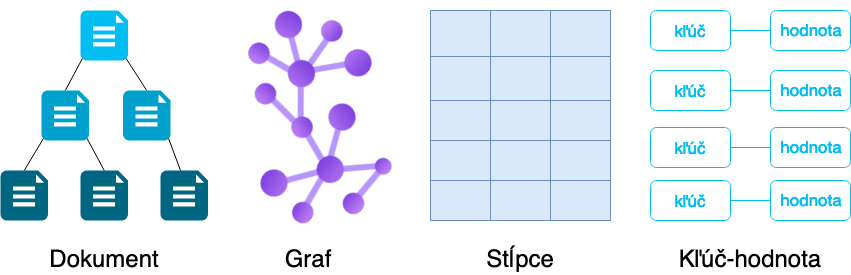
\includegraphics[scale=0.45]{obrazky/nosql_types.png}
        \caption{Ilustrácia typov NoSQL databáz \cite{nosql}.}
        \label{pic:nosql_types}
    \end{figure}

\section{Frontend}
Frontend, alebo častokrát nazývaný aj ako klient, je prezentačná vrstva aplikácie ktorá poskytuje používateľské rozhranie. Je to časť, ktorú užívateľ vidí, s ktorou pracuje a ovláda. Medzi najpopulárnejšie technológie pre vývoj frontendu patrí HTML, CSS a JavaScript, pomocou ktorých je táto aplikácia implementovaná. 

\subsection{JavaScript}
JavaScript je objektovo orientovaný skriptovací jazyk. Najviac sa používa pri vývoji dynamických webových aplikácií, ale využíva sa aj pri tvorbe multiplatformových stolových aplikácií a hybridných mobilných aplikácií. Poskytuje interaktivitu nad obsahom. 

Medzi jeho výhody patrí dynamické načítanie stránky, zmena obsahu bez fyzického znova načítania stránky a jeho rozšíriteľnosť. JavaScript sa hlavne zameriaval na klientskú časť aplikácie, kým nenastúpil na scénu framework \texttt{Node.js}(\ref{node}) a podobné serverové technológie, účelom ktorých je tvorba serverovej časti aplikácie.

Existuje niekoľko JavaScriptových frameworkov pre uľahčenie vývoja, pomocou ktorých sa vyhneme takzvaným biolerplate\footnote{Biolerplate - kód ktorý sa musí opakovane vyskytovať na viacerých miestach bez významnej zmeny} kódom. Medzi najpopulárnejšie frameworky patrí Vue.js, React, Angular a Node.js.

\subsection{Vue.js}
Vue.js\cite{vue-guide} je JavaScriptový framework, ktorý patrí medzi najpopulárnejšie nástroje pre tvorbu jednostránkových aplikácii. Je výkonný, rýchly a minimalistický. Stal sa jedným z obľúbených kvôli jeho jednoduchosti. Má veľmi prehľadnú a pestrú dokumentáciu v anglickom aj čínskom jazyku.

Framework bol vytvorený Evanom Youom, ktorý pracoval v Googli a Meteore. V Googli začal používať framework AngularJS, ktorý mu avšak nevyhovoval kvôli jeho striktnému písaniu kódu. Jeho motiváciou bolo vziať najlepšie vlastnosti Angularu a vytvoriť z nich nástroj, ktorý mu zjednoduší a zefektívni prácu.

Frontend aplikácie je implementovaný pomocou tohto frameworku. V sekcii \ref{vue} sa nachádza hlbší a podrobnejší popis jednotlivých vlastností frameworku.

\subsection{Angular}
Angular\cite{angular} je JavaScriptový open-source framework, vytvorený spoločnostou Google. Súčasná verzia sa označuje aj ako Angular 2+, ktorá má zatiaľ jedenásť podverzií. Angular funguje na báze TypeScriptu, o ktorom si povieme viac v kapitole \ref{typescript}.

\subsection{React}
React je frontendová JavaScriptová open-source\footnote{Open-source software má dostupný zdrojový kód pre verejnosť} knižnica pre tvorbu užívateľských rozhraní. Na rozdiel od podobných frameworkov ako je Angular, React\cite{react} sa sústreďuje iba na jednu špecifickú oblasť \texttt{MVC}\footnote{Model-View-Controller - softwarová architektúra, ktorá rozdeľuje aplikáciu na dátový model, užívateľské rozhranie a logiku} architektúry, a to je vrstva pohľadu (anglicky \texttt{view}). Knižnica bola predstavená v roku 2013 spoločnosťou Facebook, ktorá ju už niekoľko rokov predtým používala a vyvíjala. 

\section{Backend}
Backend, mnohokrát nazývaný aj ako server, je základom aplikácie. Tvorí časť, ktorá je skrytá pred používateľom. Jeho úlohou je prijímanie a posielanie dát pre klienta cez aplikačné rozhranie. Tieto údaje spracuje, ukladá, alebo modifikuje v databáze.

\subsection{Node.js}
Node.js\cite{nodejs} je spúšťacie prostredie(runtime environment) pre aplikácie napísané v jazyku JavaScript, mimo webového prehliadača. Je zakladaný na motore Chrome V8 JavaScript, čo znamená, že sa prostredie správa rovnako ako webový prehliadač Google Chrome. Node.js sa najčastejšia využíva pri tvorbe serverovej časti webových aplikácií.

Platforma obsahuje viacero frameworkov pre uľahčenie vývoja aplikácií, najpopulárnejším z nich je \texttt{Express.js}, pomocou ktorého je implementovaná serverová časť aplikácie. Podrobnejší popis vlastností oboch technológií sa nachádza v sekcii \ref{node}.

\subsection{Firebase}
Firebase\cite{firebase} je platforma typu \textit{backend-ako-služba} (anglicky \texttt{Backend-as-a-Service}) , ktorá bola vytvorená v roku 2011. V roku 2014 bola odkúpená spoločnosťou Google, ktorá ju doteraz vyvíja. Platforma pomáha v tvorbe, vylepšovaní a škálovaní aplikácií.

BaaS je typ cloudových služieb pre tvorbu aplikácií bez investovania do vlastnej backend infraštruktúry. Uľahčuje vývojárom prácu zapúzdrením služieb na backendu, aby sa mohli sústrediť hlavne na tvorbu frontendu. Medzi tieto služby patrí autentifikácia užívateľov, manažment databáze, monitorovanie a analýza, vzdialené aktualizácie, cloudové úložisko alebo hosting. Všetky tieto služby Firebase poskytuje. 

\subsection{PHP}
Hypertextový preprocessor\cite{php}, v skratke PHP, je populárny skriptovací jazyk, ktorý beží na strane servera. Slúži na vytváranie statických aj dynamických web stránok a aplikácií. Jazyk je bezplatný a použiteľný medzi viacerými platformami. Na PHP sa zakladá viacero frameworkov, ktoré poskytujú základnú štruktúru pre zjednodušený a zrýchlený vývoj. Medzi najpopulárnejšie patria Laravel a Symfony.

Laravel je najpopulárnejší webový PHP framework. Jeho použitie je bezplatné a má voľne dostupný zdrojový kód pre verejnosť. Laravel sa stal obľúbeným kvôli jeho rýchlosti a jednoduchosti. Umožňuje vytváranie komplexných webových aplikácií, bez ohľadu na ich rozsiahlosť. Podporuje MVC architektúru, poskytuje smerovanie, autentifikáciu užívateľov, a mnoho ďalších\cite{php}.

Symfony je jeden z najstarších a najspoľahlivejších PHP frameworkov. Je výbornou voľbou pre vysoko škálovateľné projekty. S Laravelom majú veľa podobných vlastností. Kým Symfony sa skôr zameriava na pokročilých programátorov, Laravel je jednoduchší pre nových vývojárov\cite{php}.

\subsection{Python}
Python je interpretovaný, objektovo-orientovaný programovací jazyk\cite{python}. Poskytuje dynamické typovanie premenných, ktoré je podrobnejšie rozpísané v sekcii \ref{typescript}, a rýchly vývoj aplikácií. Python patrí medzi modulárne jazyky, podporuje moduly a balíky, pomocou ktorých umožňuje znovupoužitie zdrojového kódu. Jazyk obsahuje viacero frameworkov, jedným z najpopulárnejších je Django.

Django je open-source webový framework pre vytváranie webových aplikácií. Je postavaný na princípe MTV (Model-Template-View). Obsahuje dátový model a pohľad, ktorý je posielaný do šablóny. Namiesto písaní SQL dotazov preferuje prístup ORM\footnote{ORM - Objektové relačné mapovanie}, transformáciu Python objektov na dotazy.

\section{Nástroje pre tvorbu prezentácií}
Nástroje pre tvorbu prezentácií, ďalej označované ako slideshow frameworky, sú pomôcky pre vytváranie prezentácií vo webovom prehliadači pomocou webových technológií, ako HTML, CSS a JavaScript.

\subsection{Reveal.js}
Reveal.js je najpopulárnejším nástrojom pre tvorbu prezentácií v prehliadači pomocou webových technológií. Framework je založený na čistom JavaScripte a nevyžaduje žiadny iný framework pre jeho použitie. Zdrojový kód projektu je voľne dostupný pre verejnosť. 

Prezentovanie prezentácií v tejto práci sa rieši práve cez tento nástroj, jeho podrobnejší popis a príklad použitia sa nachádza v sekcii \ref{reveal}.

\subsection{Eagle.js}
Eagle.js\footnote{\url{https://github.com/zulko/eagle.js/}} je slideshow framework založený na Vue.js. Podporuje animácie a motívy. Poskytuje užívateľom zopár komunitou vytvorených šablón pre rýchlejšiu tvorbu prezentácií. 

Nevýhodou Eagle.js je, že jeho vývoj je zanedbaný. Posledná aktualizácia bola vydaná 23.10.2019. Framework používa takzvané mixiny, ktoré sú už v najnovšej verzii Vue.js neschválené (anglicky deprecated) a nahradené \texttt{Composition API}. O mixinoch a Composition API sa čitateľ dozvie viac v sekcii \ref{compositionapi}.

\subsection{Impress.js}
Impress.js\footnote{\url{https://impress.js.org/}} je určený hlavne pre upútanie pozornosti pomocou pestrých animácií. Silnou stránkou tohto frameworku sú animácie poskytované CSS3. Nástroj je vhodný pre prezentácie s malým obsahom.

\chapter{Použité webové technológie}
\section{Databáza}
V tejto sekcii sa čitateľ zoznámi s NoSQL databázou MongoDB a knižnicou Mongoose.

\subsection{MongoDB}
\label{mongodb}
TODO

\subsection{Mongoose}
TODO

\section{TypeScript}
\label{typescript}
Aby sa porozumela logika a nápad za vytvorením TypeScriptu, je nutné sa zoznámiť s nevýhodami JavaScriptu. JavaScript\cite{typescript} umožní zo statického webu vytvoriť dynamické aplikácie, ktoré používame dodnes. Písať zdrojový kód čisto v JavaScriptu je pomerne náročné a pri väčších projektoch takmer nemožné. Samotný jazyk neumožňuje počas programovania uvádzať dátové typy, čo veľmi sťažuje napovedanie v kóde a tiež jeho automatickú kontrolu.

TypeScript\cite{typescript} bol vytvorený v roku 2012 firmou Microsoft a jeho zdrojový kód je dostupný pre verejnosť. Jedná sa o nadstavbu jazyka JavaScript. Rozširuje ho o triedy, rozhrania, statické typovanie a ďalšie funkcionality z objektovo orientovaného programovania. TypeScript je využívaný aj spoločnosťou Googlu, ktorá ho integrovala do JavasSriptového frameworku Angular.

Ako už bolo spomenuté, TypeScript umožňuje programátorom statické typovanie. Existujú dva základné typové systémy:
    \begin{itemize}
        \item Pri \textbf{dynamickom typovaní} premenná má nastavený dátový typ, ale systém typ skrýva a nedáva ho vôbec najavo. Premenné pri dynamickom typovaní mnohokrát ani nemusia byť deklarované, akonáhle sa do nejakej premennej niečo uloží a jazyk zistí, že nebola nikdy deklarovaná, sám ju založí. Do tej istej premennej sa môže ukladať reťazec, potom objekt a potom pole. Jazyky využívajúce dynamický typovanie vnútorne automaticky menia dátový typ. V týchto jazykoch je vývoj rýchlejší vďaka menšiemu množstvu kódu, zástupcovia sú napríklad Python, alebo práve JavaScript.
        \item Pri \textbf{statickom typovaní} je striktne vyžadované definovanie typu premennej a typ je naďalej nemenný. Pri uložení hodnoty iného typu do premennej, kompilácia zdrojového kódu skončí chybovím hlásením.
    \end{itemize}
    
    TypeScript\cite{typescript} je typizovaním jazykom, všetky premenné musia byť najprv deklarované s priradeným dátovým typom. Nevýhodou je, že vďaka deklaráciám je zdrojový kód objemnejší a vývoj pomalší. Naopak obrovskou výhodou je, že kompilátor pred spustením skontroluje, či všetky nastavené hodnoty vyhovujú ich dátovým typom. Dynamické typovanie síce vyzerá ako výhodné, ale pri čítaní zdrojového kódu je ťažké zistiť typ hodnoty premennej. TypeScript do základnej mieri tiež povoľuje využitie dynamických typov cez takzvané \texttt{union typy}. Union typy umožňujú nastavenie viacero dátových typov premennej, napríklad \texttt{let data: string | number}, kde premenná \texttt{data} môže obsahovať reťazec, alebo číslo. TypeScript pri priradení hodnoty nesprávneho dátového typu nedovolí program ani skompilovať a na chybu ihneď upozorní.
\section{Frontend}
TODO

\subsection{HTML}
Hypertextový značkovací jazyk\cite{html}, alebo skrátene HTML je jazyk vytvorený Timom Berners-Leeom v roku 1991. Avšak nie je to programovací jazyk, neumožňuje vytváranie premenných, alebo funkcií. Jazyk je určený na vytváranie webových stránok, na organizovanie a formátovanie rôznych informácií zobraziteľných vo webovom prehliadači. Umožňuje užívateľom vytvárať a štrukturovať sekcie, nadpisy, paragrafy, odkazy a mnoho ďalších pre webové stránky a aplikácie. Pri práci s HTML sa používajú štruktúry, ktoré sa nazývajú značky\texttt{(tagy)} a \texttt{atribúty}, pomocou ktorých sa štrukturujú jednotlivé časti web stránky. 

\subsection{CSS}
TODO

\subsection{Vue.js}
Vue.js\cite{vue-guide} patrí medzi najpopulárnejšie nástroje pre tvorbu Single Page Aplikácií. Je výkonný, rýchly a minimalistický. Veľkou výhodou je, že patrí medzi progresívne frameworky, našu aplikáciu vieme rozdeliť na viacero častí, ktoré môžu byť samostatne vyvíjané. Stal sa jedným z obľúbených kvôli jeho jednoduchosti. Má veľmi prehľadnú a pestrú dokumentáciu v anglickom aj čínskom jazyku.

Framework bol vytvorený Evanom Youom, ktorý pracoval v Googlu a Meteoru. V Googlu začal používať AngularJS, ktorým sa inšpiroval, ale tento framework mu nevyhovoval kvôli jeho striktnému písaniu kódu. Jeho motiváciou bolo vziať najlepšie vlastnosti Angularu a vytvoriť z nich nástroj, ktorý mu zjednoduší a zefektívni prácu.

Dizajn Vue.js sa inšpiroval MVVM\footnote{Model-View-ViewModel} architektúrou. Zameriava sa na vrstvu pohľadu. Spája pohľad a model cez dvojstrannú väzbu (anglicky two-way binding), ako je vidieť na obrázku \ref{pic:mvvm}. Ostatné funkcionality SPA, ako smerovanie a úložisko(ďalej označované ako store) môžu byť doplnené cez pomocné knižnice.
    \begin{figure}[!hbt]
        \centering
        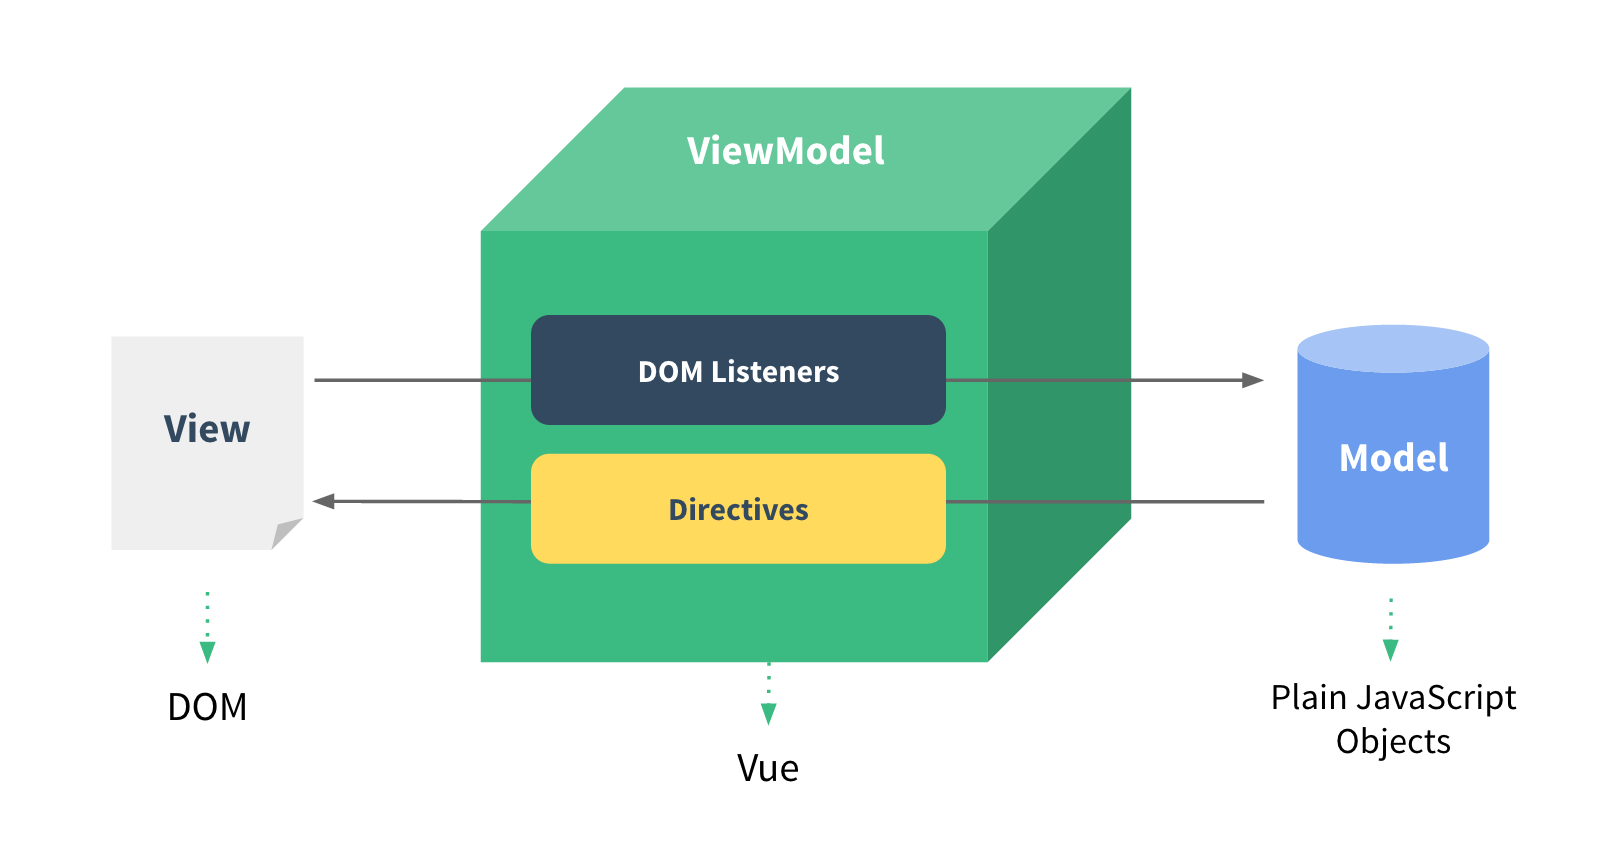
\includegraphics[scale=0.2]{obrazky/mvvm.png}
        \caption{Znázornenie úlohy Vue.js v MVVM architektúre \cite{vue-guide}.}
        \label{pic:mvvm}
    \end{figure}

\subsection*{Inštalácia}
Vue.js bol vytvorený aby bol ľahko osvojiteľný a a použiteľný. Môže byť začlenený do projektu viacerými spôsobmi. 

Štyri hlavné spôsoby sú nasledovné:
    \begin{itemize}
        \item Importovanie balíčka do HTML stránky cez CDN:
        \begin{verbatim}<script src="https://unpkg.com/vue@next"></script>\end{verbatim}
        \item Stiahnutie JavaScriptových súborov a importovanie ich rovnakým spôsobom ako u CDN
        \item Inštalácia cez správcu balíčkov npm
        \item Použitie oficiálneho CLI pre zkonštruovanie projektu
    \end{itemize}
    
\subsection*{Komponenty}
Komponenty hrajú vo Vue.js veľmi dôležitú rolu, umožňujú tvorbu vysoko škálovateľnej aplikácie, ktorá je poskladaná z malých a znovupoužiteľných častí. Môžeme mať komponenty napríklad pre hlavičku, bočný panel, obsah, ktoré môžu obsahovať ďalšie komponenty pre zoznam prezentácií, výpis detailu prezentácie. Výsledkom rozdelenia do jednotlivých častí je ľahko udržateľný a prehľadný zdrojový kód. Komponenty tvarujú hierarchiu vnoreného stromu, ktorý je znázornený na obrázku \ref{pic:components}. Tento strom reprezentuje aplikačné rozhranie.
    \begin{figure}[!hbt]
        \centering
        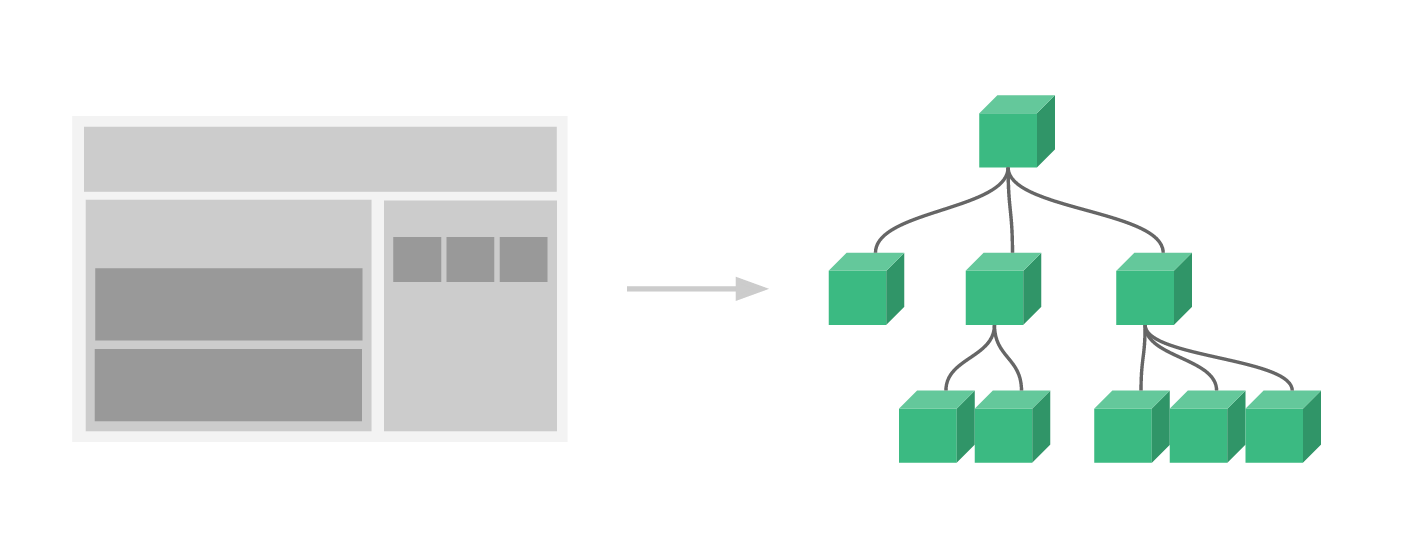
\includegraphics[scale=0.25]{obrazky/components.png}
        \caption{Znázornenie komponentov ako vnorený strom\cite{vue-guide}.}
        \label{pic:components}
    \end{figure}
    
\subsection*{Registrovanie komponentov}
Existujú dva postupy registrovania jednotlivých komponentov: \textit{lokálne} a \textit{globálne}. Lokálne komponenty je potrebné pred každým použitím importovať, narozdiel od globálnych, ktoré stačí zaregistrovať raz a môžu byť použité v šablóne hociktorej komponenty. 

Typický príklad pre globálnu komponentu je dizajnový prvok ako napríklad animácia pri načítaní údajov, takzvaný spinner. Tento typ animácie sa používa pri každom načítaní údajov, na viacerých miestach v aplikácii. Aby sme ho nemuseli po každom importovať stačí keď si ho raz globálne zaregistrujeme a môžme ho voľne používať. 

Príklad lokálnej komponenty je formulár pre registrovanie užívateľa, ktorý sa pravdepodobne použije iba raz a nepotrebujeme ho mať dostupný v celej aplikácii.

\subsection*{Komunikácia medzi komponentami}
Komponenty začnú byť viac užitočné pri vymieňaní údajov medzi sebou. Štandardne, každá jedna je izolovaná, čo znamená, že nemá prístup k rodičovským údajom. Majme komponentu pre stručný výpis informácií o prezentácii, po kliknutí na ňu sa zobrazí ďalšia komponenta s detailným výpisom. Pri tomto príklade potrebujeme predať informácie o prezentácii z jednej komponenty na druhú. Na komunikáciu medzi rodičom a potomkom sa používa \texttt{props} a metóda \texttt{\$emit}.

Props sú atribúty, ktorým vieme nastaviť hodnoty. Slúžia na predanie údajov z rodiča na potomka. Po nadobudnutí hodnoty sa z nich stanú premenné použiteľné v komponente. Počet props nie je obmedzený a prijíma ľubovolný typ údajov.

Metóda \$emit slúži na komunikáciu opačným smerom. Pomocou tejto metódy vieme vytvoriť vlastnú udalosť, ktorú rodič môže odpočúvať. Majme komponentu potomka v ktorej sa nachádza tlačítko. Kliknutím na tlačítko sa zavolá metóda \$emit do ktorej sa predá meno udalosti a ľubovolný údaj. Rodičovská komponenta môže odchytiť túto udalosť a reagovať na ňu. Vysielanie udalostí je užitočné keď máme viacero potomkov s rovnakou logikou, týmto spôsobom nemusia všetky tieto komponenty obsahovať tú istú logiku, stačí keď bude implementovaná iba v rodičovskej komponente a pristúpi sa k nej cez \$emit.

\subsection*{Životný cyklus komponenty}
Vo Vue.js každá komponenta je samostatná Vue inštancia\footnote{Jeden konkrétny exemplár triedy} a každá inštancia má svoj životný cyklus. Životný cyklus komponenty sa skladá z niekoľkých krokov, ako napríklad jej vytvorenie, pripevnenie inštancie k DOM\footnote{Objektový model HTML dokumentu}, aktualizácia DOM-u pri zmene údajov alebo jej zrušenie. Vývojári majú pri každom kroku možnosť pridania vlastného kódu cez funkcie \texttt{lifecycle hooks}. Medzi najpoužívanejšie patria:
    \begin{itemize}
        \item\texttt{beforeCreated} - Volá sa hneď po inicializácii inštancie, ktorá zatiaľ nič neobsahuje.
        \item\texttt{created} - Pri tomto kroku sa dokončilo nastavenie pozorovania dát, computed premenných, metód a udalostí. Zatiaľ nemáme prístup k DOM. Môže sa použiť pre registrovanie vlastných udalostí.
        \item\texttt{beforeMount} - Volá sa pred pripevnením DOM.
        \item\texttt{mounted} - Najpoužívanejšia funkcia lifecycle hook. Volá sa po pripevnení inštancie k DOM. V tejto funkcii už máme prístup k jednotlivým elementom v DOM. Častokrát používaná pre sťahovanie dát z API.
        \item\texttt{beforeUpdate} - Volá sa pri zmene dát. Máme prístup k existujúcemu DOM pred jeho aktualizáciou.
        \item\texttt{updated} - Funkcia volaná po znova-vykreslení DOM.
        \item\texttt{beforeUnmount} - Volá sa pred odpojením inštancie od DOM-u.
        \item\texttt{unmounted} - Po tomto kroku je inštancia kompletne odpojená, taktiež jej potomky a udalosti. Používaná pre odpojenie vlastných udalostí.
    \end{itemize}

Pri použití Composition API, o ktorom si povieme viac v sekcii \ref{compositionapi}, sa tieto funkcie trochu líšia. Lifecycle hooky beforeCreated a created sú súčasťou funkcie \texttt{setup()} a pred každý hook treba pridať predponu \texttt{on}: onCreated, onMounted, atď. 

    \begin{figure}[!hbt]
        \centering
        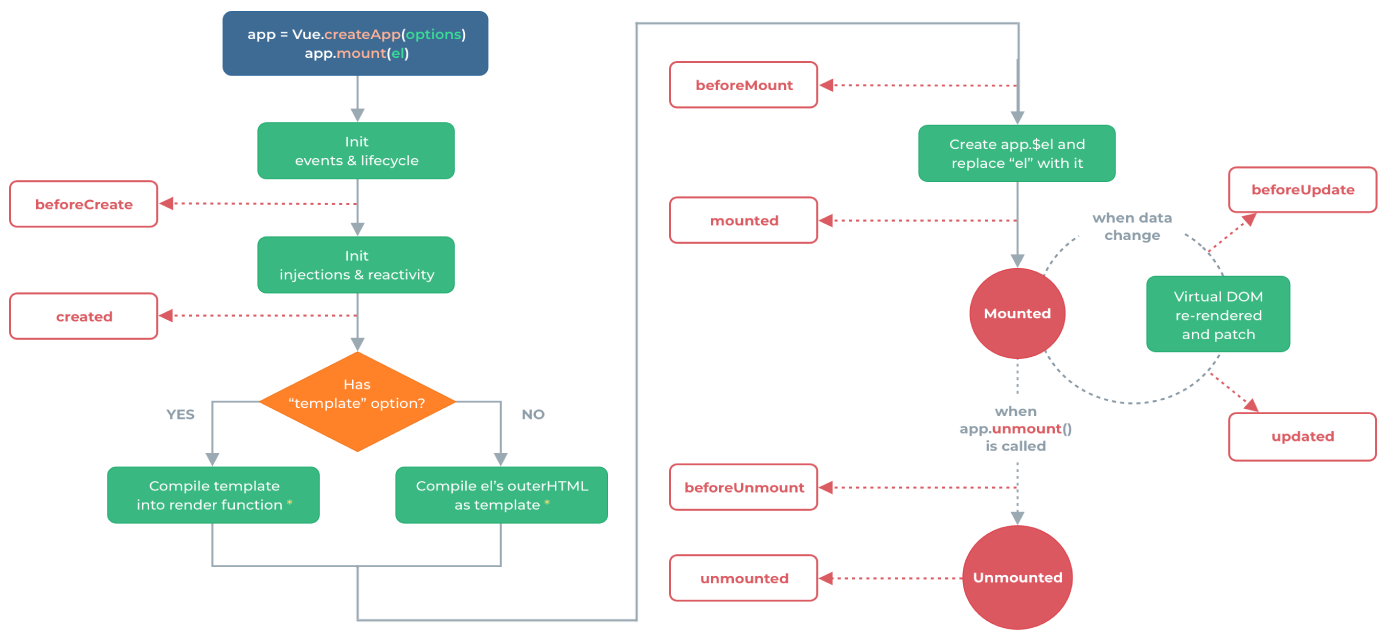
\includegraphics[scale=0.3]{obrazky/lifecycle.png}
        \caption{Graf životného cyklu komponenty\cite{vue-guide}.}
        \label{pic:components}
    \end{figure}

\subsection*{Šablóna}
Komponenta sa vykresľuje cez HTML šablónu. Okrem základnej funkcionality jazyka HTML umožňuje aj výpis statických aj dynamických hodnôt, dynamickú aktualizáciu CSS štýlov a tried, použitie podmienok na obmedzenie vykresľovania a použitie cyklov pre prechádzanie hodnôt v poli. V šablóna má vývojár prístup k premenným aj metódam. Obsah šablóny sa musí nachádzať medzi značkou \texttt{<template>}.

\subsection{Composition API}
\label{compositionapi}
TODO

\subsection{Nuxt.js}
TODO

\subsection{Reveal.js}
TODO

\subsection{Ostatné balíčky a knižnice}
TODO

\section{Backend}
TODO

\subsection{Node.js a Express.js}
\label{node}
TODO

\subsection{Aplikačné rozhranie}
TODO

\subsection{Ostatné balíčky a knižnice}
TODO
\chapter{Návrh riešenia}
V tejto kapitole sa čitateľ zoznámi s návrhom celej aplikácie. V prvej sekcii sú rozobrané prípady použitia aplikácie. Ďalej sa čitateľ dočíta o návrhu architektúry systému, o návrhu užívateľského rozhrania, o návrhu databáze a na záver o návrhu serverovej aj klientskej časti aplikácie.

\section{Použitie aplikácie}
Pri príchode na webovú stránku sa užívateľ ocitne na autentifikačnej stránka kde sa musí prihlásiť, alebo zaregistrovať, aby mohol postúpiť ďalej.

Po úspešnom prihlásení užívateľ je presmerovaný na domovskú stránku. Na domovskej stránke má prístup k zoznamu vlastných prezentácií, ktoré už vytvoril. Vie si tu vytvoriť novú prezentáciu kliknutím na tlačítko \texttt{Create New}, alebo sa odhlásiť tlačítkom \texttt{Logout}. Zoznam obsahuje kartičky jednotlivých prezentácií so stručným opisom informácií. Užívateľ si vie zobraziť prezentáciu v prezentačnom móde cez tlačítko \texttt{View}, upraviť poslednú verziu cez tlačítko \texttt{Edit} a odstrániť celú prezentáciu tlačítkom \texttt{Delete}. Kliknutím na kartičku si vie zobraziť detailný popis prezentácie. V detailu má prístup k vytvoreným verziám a popisom k nim. Nachádza sa tu náhľad do stránok jednotlivých verzií pre uľahčenie voľby správnej verzie.

Pri vytváraní novej prezentácie, alebo upravovaní už existujúcej nás aplikácie presmeruje na stránku editora. Editor obsahuje mnoho užitočných nástrojov pre zjednodušenie tvorby pomocou jazyka Markdown, ako napríklad typografické nástroje, vloženie zoznamov, tabuliek, obrázkov, odkazov a častí zdrojového kódu. Veľkou výhodou je výskyt náhľadu v editore, kde je hneď vidieť sformátovaný obsah stránky. V bočnom panelu má užívateľ možnosť sa vrátiť na domovskú stránku cez tlačítko \texttt{Home}. Po kliknutí na tlačítko \texttt{Save} sa zobrazí panel na uloženie prezentácie. Pri upravovaní prezentácie aplikácia ponúka úpravu názvu a pridanie popisu k verzii. Prezentáciu vie tvorca uložiť pod novou verziou, alebo môže aktualizovať práve upravovanú verziu. Kliknutím na tlačítko \texttt{Preview} sa aplikácia prepne do prezentačného módu. Prepínanie stránok v prezentačnom móde funguje pomocou klávesnicových šípok. 

Tvorca si vie zobraziť panel so stránkami cez tlačítko \texttt{Slides}. Panel obsahuje zoznam jednotlivých stránok prezentácie. Ich poradie môže byť upravené pomocou technológie ťahaj-a-pusti (anglicky drag-and-drop). Užívateľ má možnosť prepnutia zoznamu stránok do mriežkového pohľadu(anglicky grid view), kde sa dá jednoduchšie orientovať a usporiadať jednotlivé stránky. Aplikácia umožňuje kopírovanie stránok medzi prezentáciami jednoduchým kliknutím na tlačítka \texttt{Kopírovať} a \texttt{Prilepiť}.

\section{Architektúra aplikácie}
Aplikácia je rozdelená na dve časti, na klientskú a serverovú. Jedná sa o takzvanú dvojvrstvovú architektúru \texttt{klient-server}. Klientská časť sa nazýva aj ako prezentačná vrstva. Poskytuje interaktivitu užívateľom, má za úlohu zobrazovanie obsahu a údajov získaných zo servera. Zbiera užívateľom zadané dáta cez rôzne vstupy. Tieto dáta môžu byť spracovávané a upravované už na klientovi a sú posielané na server cez protokol HTTP\footnote{Hypertextový prenosový protokol} pomocou knihovne \textit{axios}. Server údaje prijíma a ďalej spracováva. Medzi úlohy serverovej časti patria: prijímanie požiadavkov od klienta, posielanie odpovedí na požiadavky stavovými kódmi a údajmi, zabezpečenie a udržovanie komunikácie cez autentifikáciu a autorizáciu užívateľov, vykonávanie rôznych výpočtov, formátovanie údajov pre databázu, alebo klienta. Klient nekomunikuje priamo s databázou, na to slúži server. Server údaje od klienta upravuje, aby vyhovovali formátu v databáze. Taktiež si vypýta dáta z databáze, ktoré spracováva a posiela klientovi. Grafické znázornenie architektúry pre jednoduchšie pochopenie sa nachádza na obrázku \ref{pic:architektura}.

    \begin{figure}[!hbt]
        \centering
        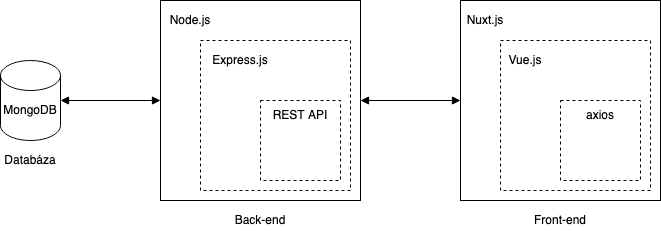
\includegraphics[scale=0.6]{obrazky/architektura.png}
        \caption{Znázornenie architektúry aplikácie.}
        \label{pic:architektura}
    \end{figure}
    
\section{Návrh frontendu}
V aplikácii sa využíva framework Nuxt.js, ktorý je nadstavbou Vue.js. Nuxt.js uľahčuje vývoj jednostránkových aplikácií a poskytuje vývojárom lepší zážitok pri programovaní. 
Aktuálne stabilná verzia Vue.js a Nuxt.js pri začatí projektu je verzia 2, ale v aplikácii sa už využívajú \texttt{composition-api} vlastnosti verzie 3, ktoré je potrebné nainštalovať ako balík cez NPM a pridať medzi moduly Nuxt.js v konfiguračnom súbore.

\subsection{Pohľad aplikácie}
Pohľad v Nuxt.js aplikácii sa skladá z viacerých vrstiev. Najvyššia vrstva je HTML súbor \texttt{App.html}, ktorý je vytvorený automaticky a slúži pre vytvorenie kostry aplikácie. Tento súbor obsahuje všetok obsah, atribúty pre hlavičku a telo HTML dokumentu. 

Nižšia vrstva obsahuje šablónu aplikácie, pomocou ktorej sa zadefinuje rovnaký obsah na viacerých stránkach. Dobrým príkladom pre obsah v šablóne je navbar, ktorý môže byť dostupný na viacerých stránkach aplikácie. 

Pod šablónou sa nachádzajú komponenty jednotlivých stránok aplikácie. Každá stránka je samostatná Vue komponenta ku ktorým Nuxt.js prideľuje špeciálne atribúty a funkcie. Medzi ne patrí \textbf{useFetch}, funkcia pre asynchrónne sťahovanie dát hneď pri návšteve stránky, naďalej atribút \textbf{auth} vyžadujúci autentifikáciu pre navštívenie stránky, alebo atribút \textbf{layout} určujúci ktorú šablónu má stránka využívať.

Každá stránka môže mať niekoľko potomkov. Potomok má rovnakú štruktúru ako rodičovská stránka a taktiež obsahuje Nuxtom pridelené atribúty a funkcie. Stránka sa môže skladať z viacerých komponentov, ich výhody už boli v tejto práci zmienené vyššie.

    \begin{figure}[!hbt]
        \centering
        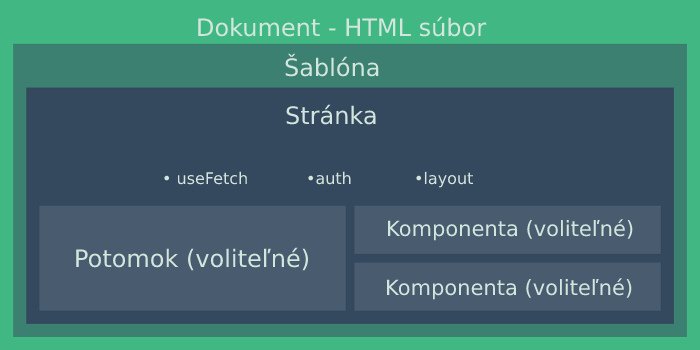
\includegraphics[scale=0.5]{obrazky/nuxt_struktura.png}
        \caption{Kompozícia pohľadu v Nuxt.js.}
        \label{pic:nuxt_strukture}
    \end{figure}


\subsection{Užívateľské rozhranie}
Užívateľské rozhranie je dôležitou súčasťou aplikácie. Je to čast s ktorou užívateľ pracuje a preto je dôležité, aby orientácia na nej bola čím jednoduchšia a prehľadnejšia. Cieľom bolo vytvoriť minimalistické rozhranie na ktorom sa ľahko nájdu potrebné ovládacie prvky.

Prototyp rozhrania bol vytvorený pomocou návrhového programu Adobe XD. Prví návrh domovskej stránky a editora je vidieť na obrázku \ref{pic:prototyp_domovska_stranka} a \ref{pic:prototyp_editor}. Odvtedy aplikácia prešla viacerým prerobaniam a dizajn sa výrazne zmenil.

\begin{figure}[!hbt]
\centering
\begin{minipage}{.5\textwidth}
  \centering
  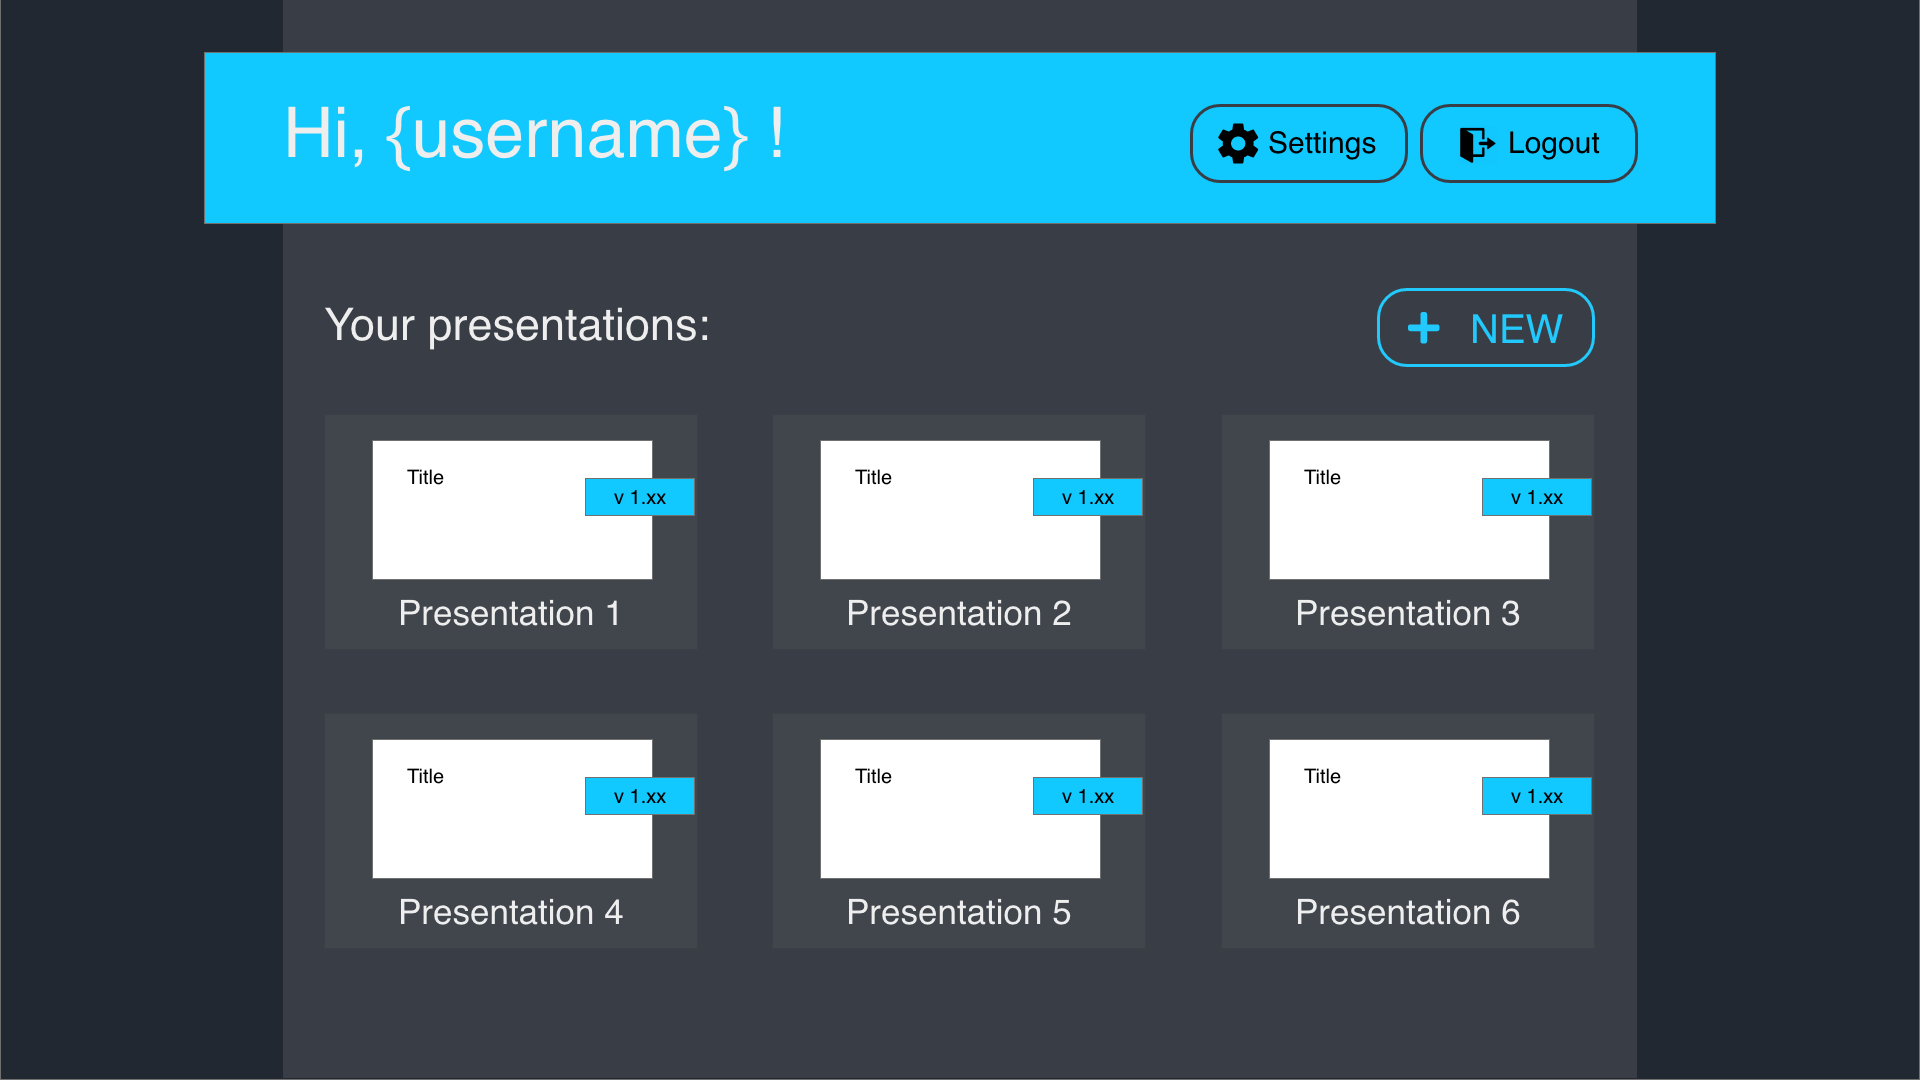
\includegraphics[scale=0.1]{obrazky/prototyp_domovska_stranka.png}
  \caption{Prototyp domovskej stránky}
  \label{pic:prototyp_domovska_stranka}
\end{minipage}%
\begin{minipage}{.5\textwidth}
  \centering
  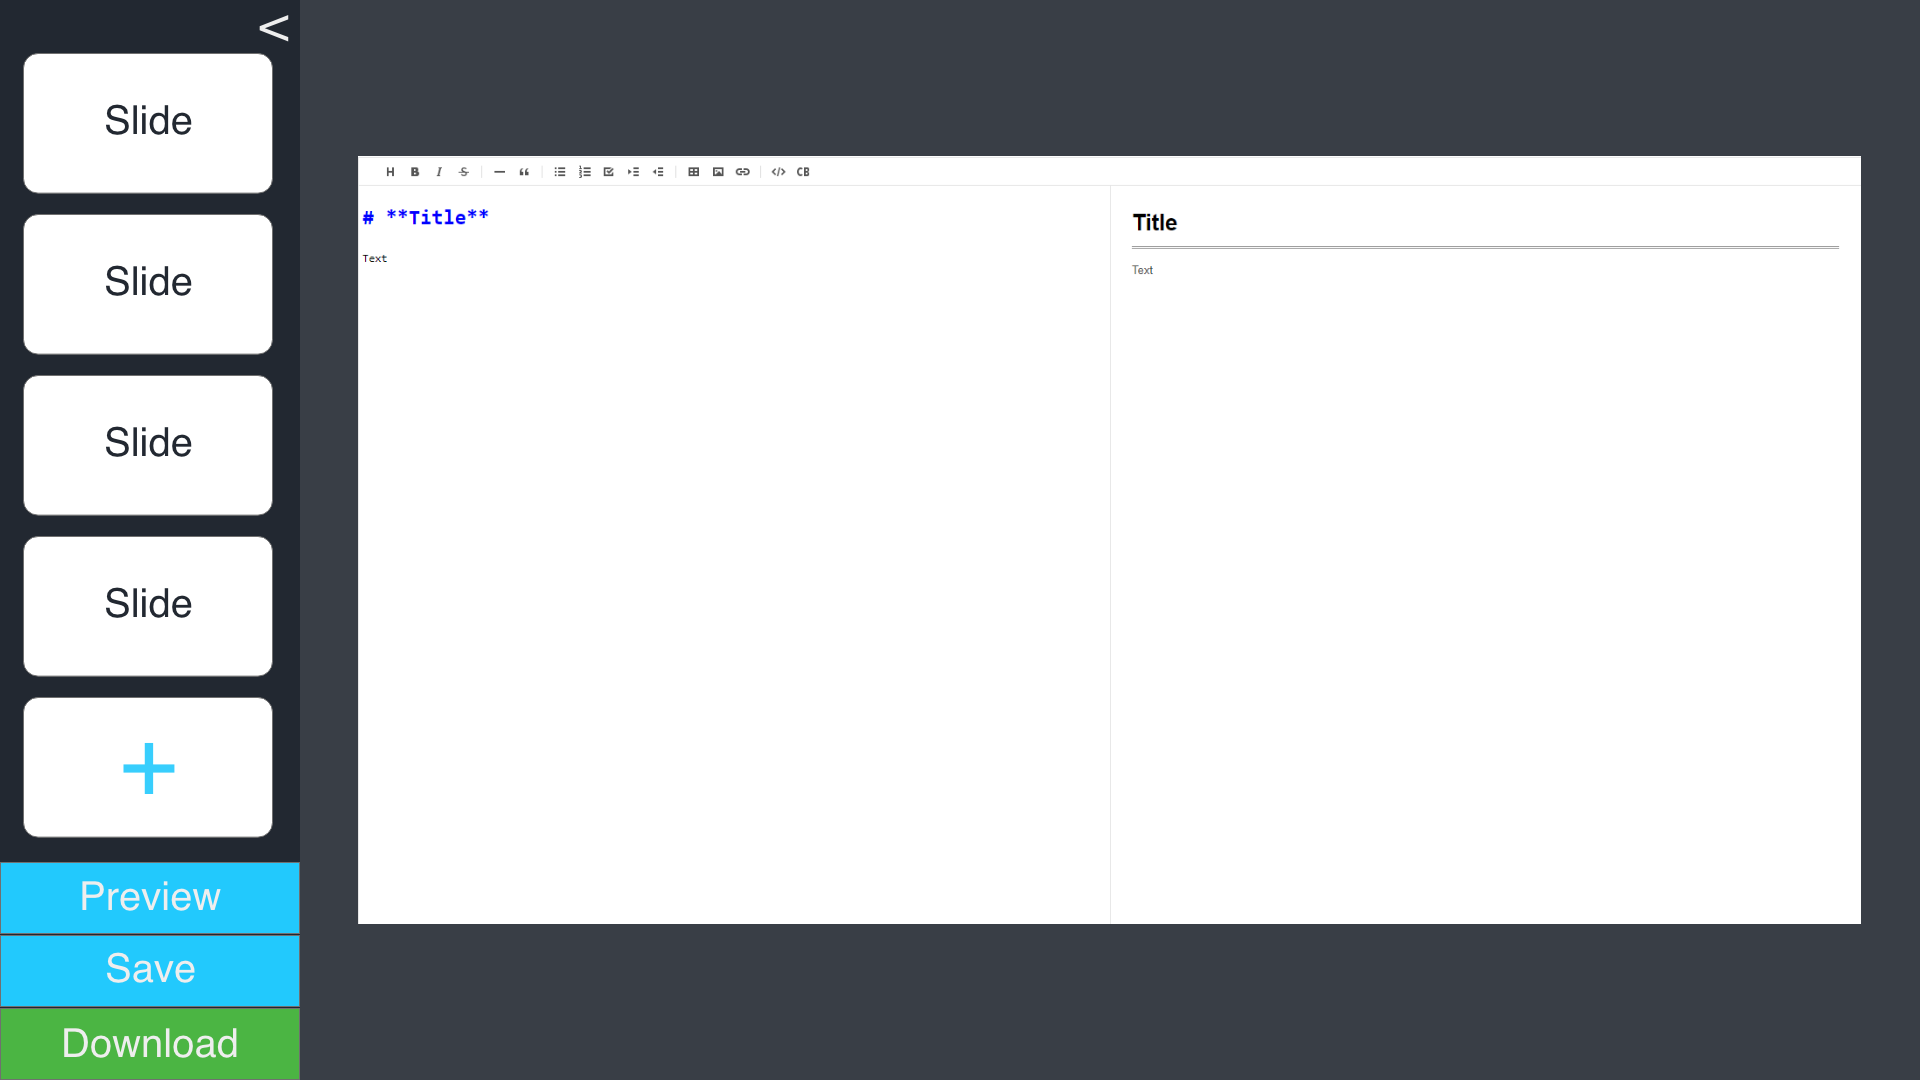
\includegraphics[scale=0.1]{obrazky/prototyp_editor.png}
  \caption{Prototyp editora}
  \label{pic:prototyp_editor}
\end{minipage}
\end{figure}

\subsection*{Autentifikačná stránka}
Autentifikačná stránka je prvá stránka na ktorej sa užívateľ ocitne pri prvom navštívení aplikácie. Stránka obsahuje prihlasovací panel, kde je nutné zadať správny e-mail a heslo. Pri novom užívateľovi je najprv nutná registrácia cez registračný panel. Aplikácia vyžaduje iba potrebné užívateľské údaje, ako meno, e-mail a heslo.

\subsection*{Domovská stránka}
Po úspešnom prihlásení sa zobrazí domovská stránka. Domovská stránka by mala obsahovať všetky potrebné informácie pre užívateľa. Stránka je znázornená na obrázku \ref{pic:domovska_stranka}. Obsahuje tlačítko pre odhlásenie a vytvorenie novej prezentácie. Nachádza sa tu zoznam vytvorených prezentácií a tlačítka pre ich spravovanie. 

Po kliknutí na hociktorý prvok zoznamu sa zobrazí detail prezentácie. Cieľom bolo vytvoriť panel kde sa tvorca vie dozvedieť všetko o daných verziách prezentácie bez toho, aby musel otvoriť editor. Vie si tu zvoliť danú verziu a má náhľad k jej stránkam, ktoré si môže voľne preklikať.

\begin{figure}[!hbt]
\centering
\begin{minipage}{.5\textwidth}
  \centering
  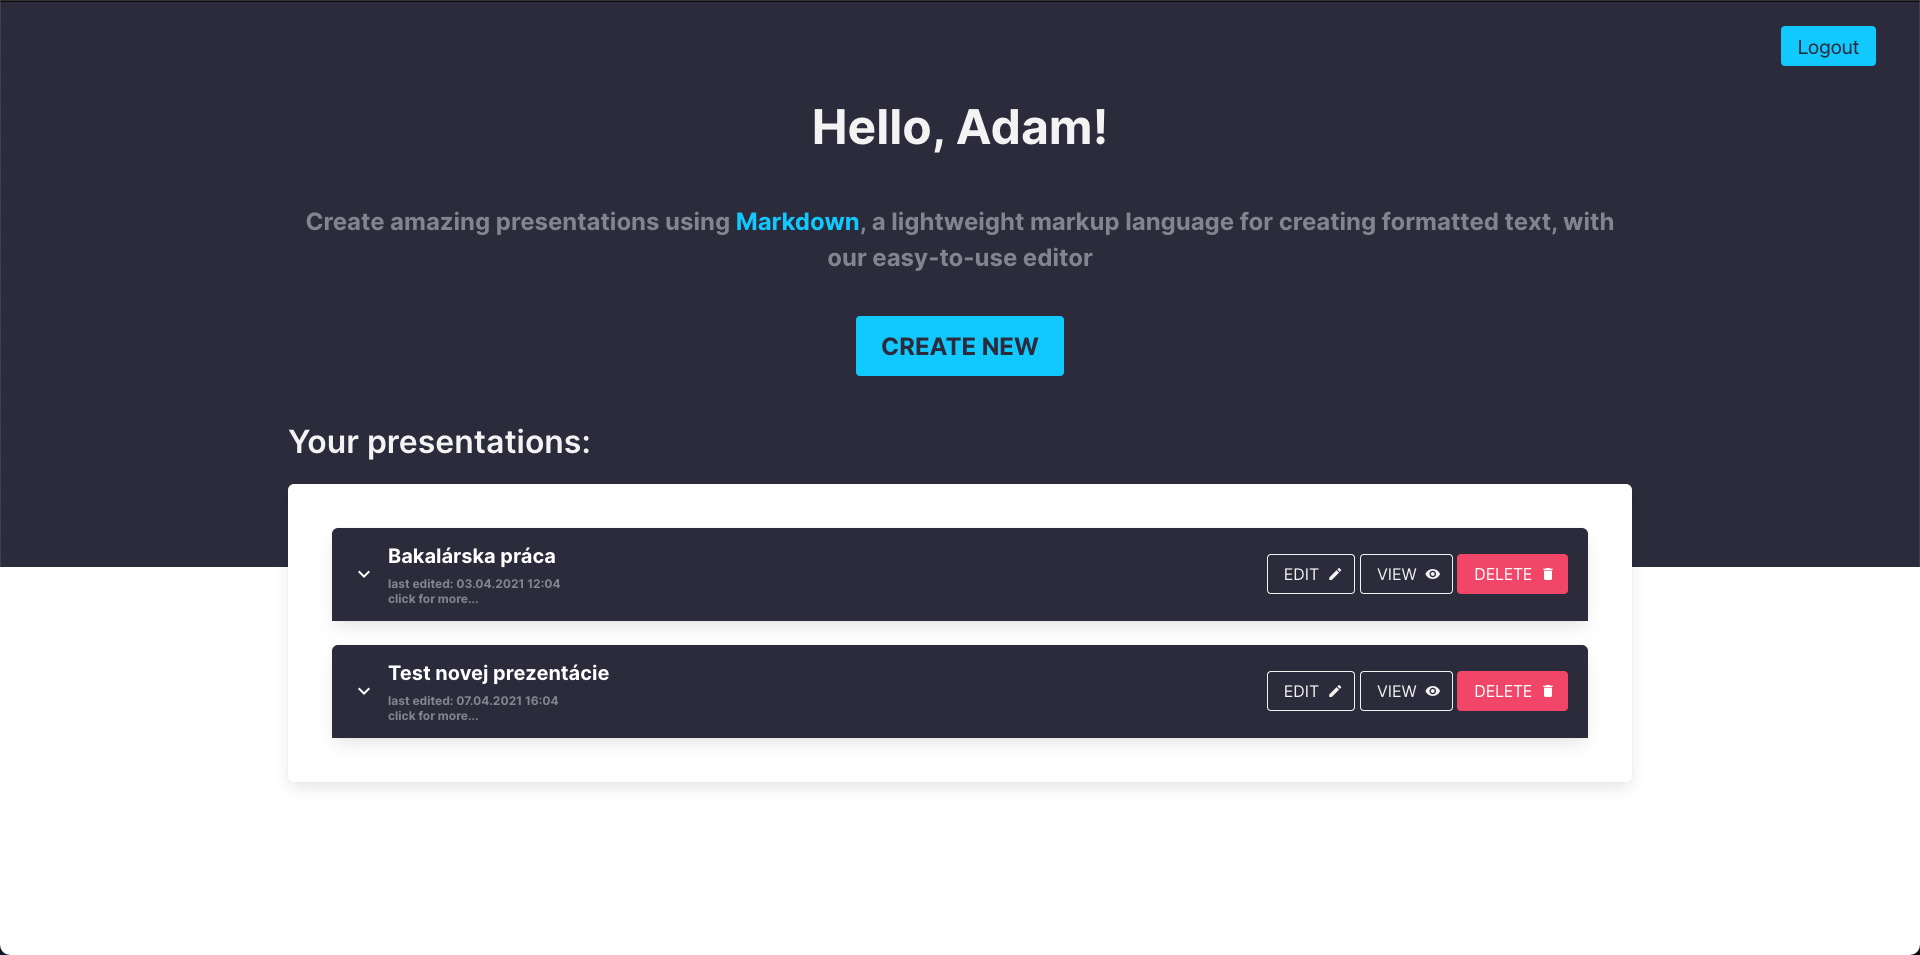
\includegraphics[scale=0.1]{obrazky/domovska_stranka.png}
  \caption{Domovská stránka}
  \label{pic:domovska_stranka}
\end{minipage}%
\begin{minipage}{.5\textwidth}
  \centering
  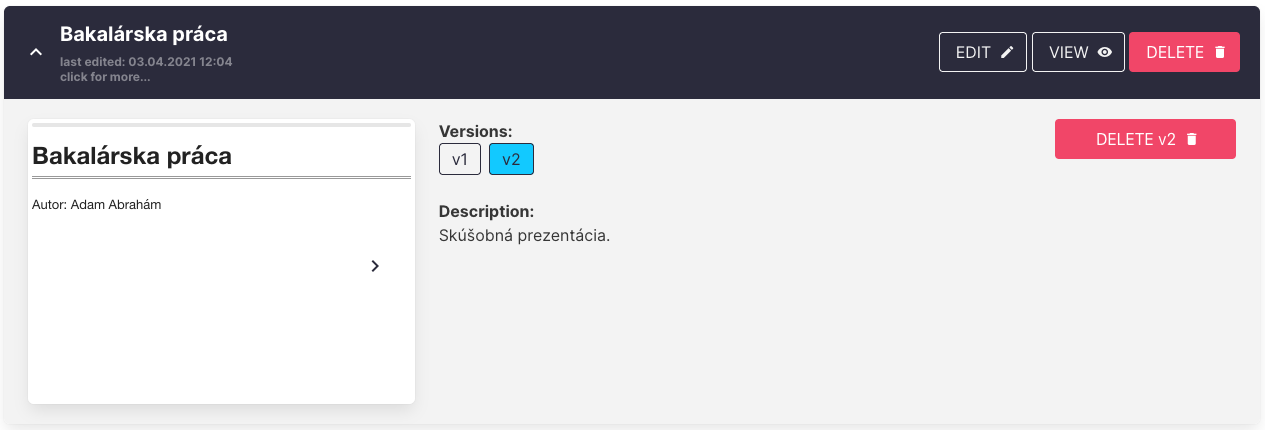
\includegraphics[scale=0.15]{obrazky/detail_prezentacie.png}
  \caption{Panel detailu prezentácie}
  \label{pic:detail_prezentacie}
\end{minipage}
\end{figure}

\subsection*{Editor}
Hlavným cieľom pri návrhu editora bolo vytvorenie stránky s čo najväčším priestorom pre písanie obsahu a náhľadom sformátovanej stránky (viz. obrázok \ref{pic:editor}). Avšak dôležité bolo správne umiestnenie nástrojov. Nástroje a ovládacie prvky by mali byť jednoducho prístupné pre tvorcu prezentácie a nemali by byť príliš schované. Pre dosiahnutie veľkého priestoru pre obsah s jednoducho prístupnými ovládacími prvkami sa navrhol vysúvací bočný panel.

Bočný panel v zavretom stave zaberá minimum priestoru na stránke a obsahuje hlavné tlačítka pre spravovanie prezentácie. Zobrazením stránok prezentácie sa bočný panel rozšíri, ako je vidieť na obrázku \ref{pic:bocny_panel}. V rozšírenom režime má tvorca prístup k zoznamu stránok, ktorý si môže zobraziť aj cez mriežkový pohľad pre jednoduchšiu orientáciu. Nad zoznamom sú dostupné tlačítka pre prácu so stránkami.

\begin{figure}[!hbt]
\centering
\begin{minipage}{.5\textwidth}
  \centering
  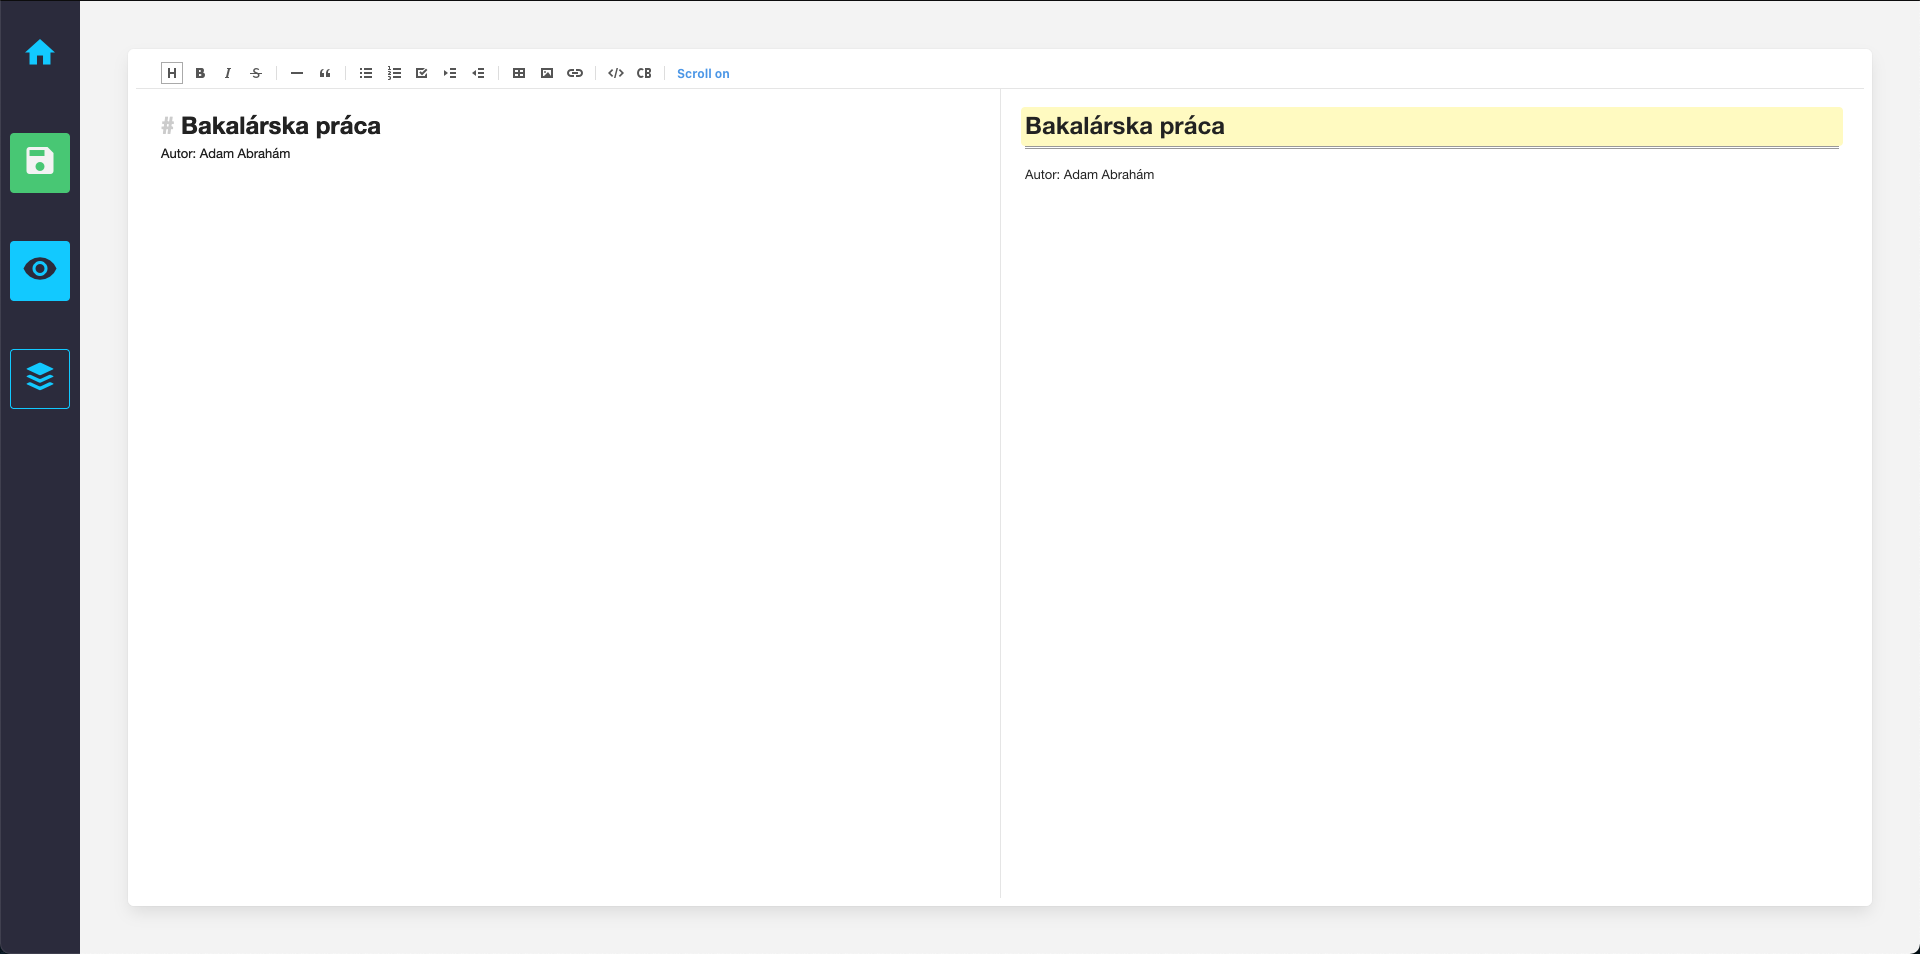
\includegraphics[scale=0.11]{obrazky/editor.png}
  \caption{Editor}
  \label{pic:editor}
\end{minipage}%
\begin{minipage}{.5\textwidth}
  \centering
  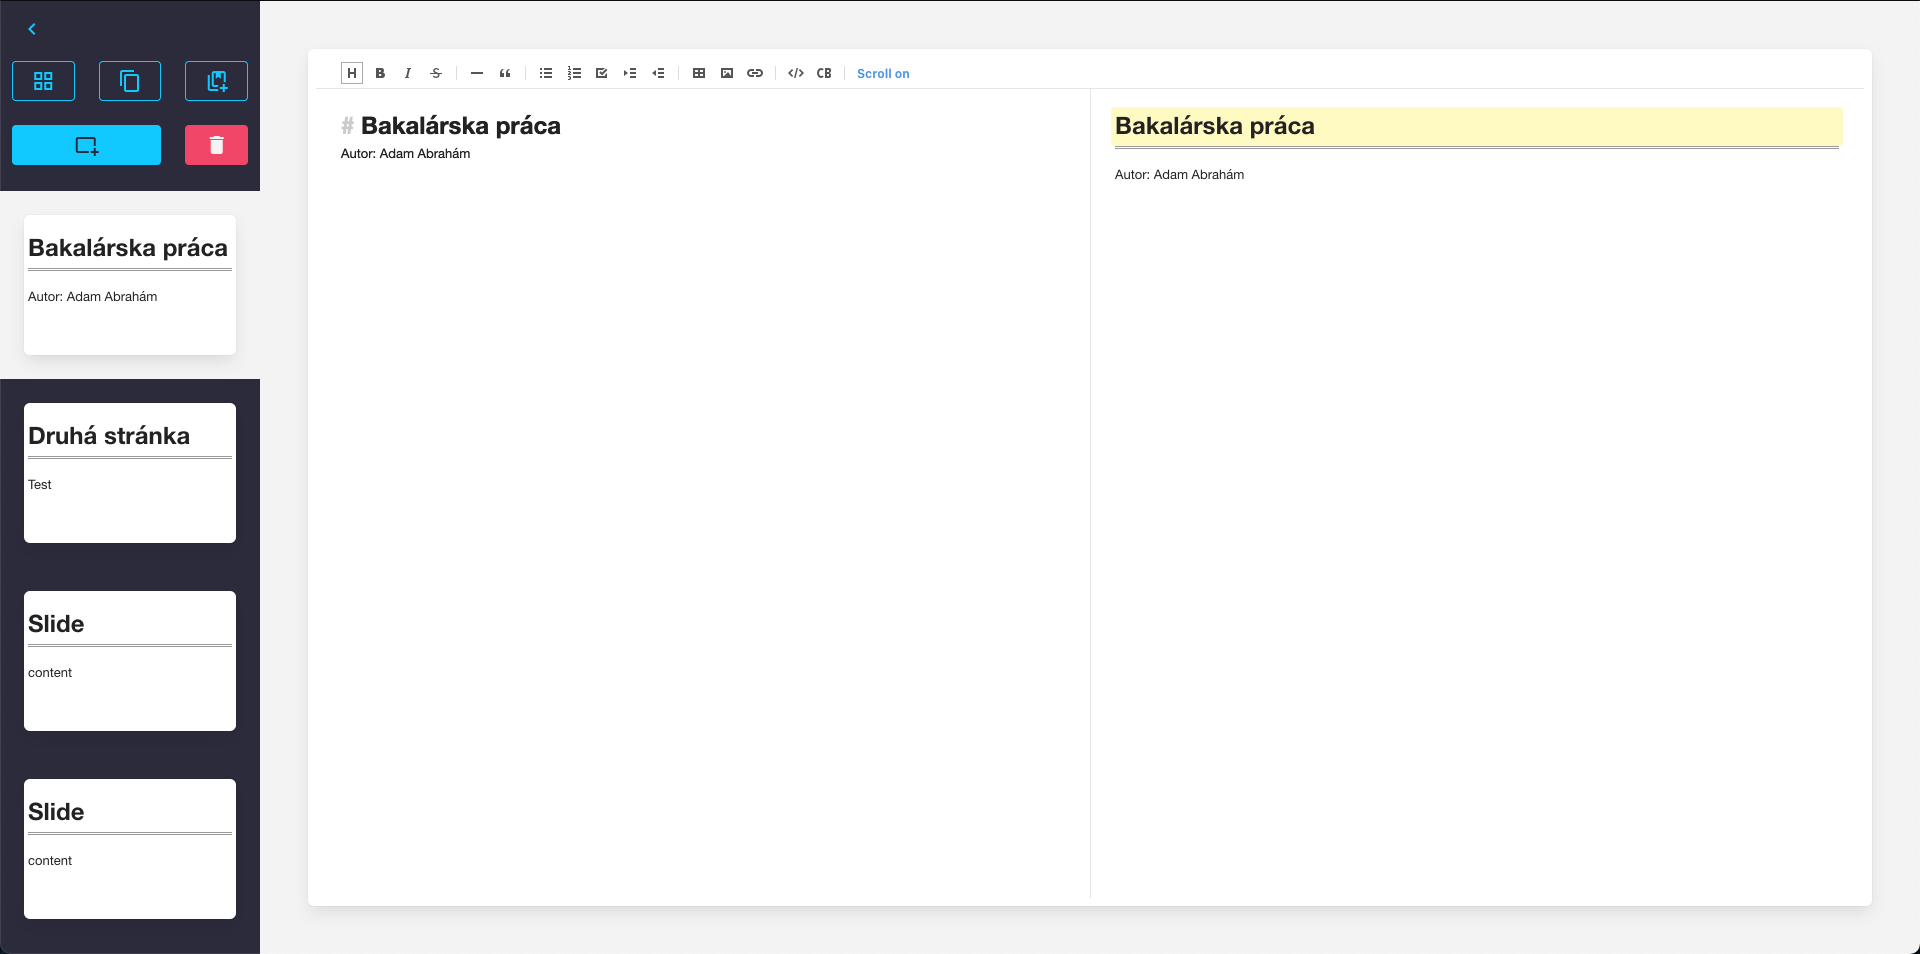
\includegraphics[scale=0.11]{obrazky/bocny_panel.png}
  \caption{Rozšírený bočný panel}
  \label{pic:bocny_panel}
\end{minipage}
\end{figure}

\subsection*{Stránka prezentácie}
Do prezentačného režimu sa užívateľ môže dostať cez domovskú stránku, ale aj cez editor. Na stránke je znázornený obsah prezentácie na celej obrazovke. Prezentácia je v tomto režime interaktívna a umožňuje prepínanie strán cez šípky klávesnice.

\section{Návrh databáze}
V tejto sekcii sa nachádza popis zvolených produktov pre databázu a popis uchovávanie údajov. Databáza obsahuje dve kolekcie. Nižšie sa nachádza popis oboch kolekcií a ich využitie v aplikácii. Pre jednoduchšie pochopenie, grafické znázornenie návrhu databáze je vidieť na obrázku \ref{pic:database}

\subsection*{MongoDB Atlas}
Na spravovanie a hosťovanie údajov sa používa cloudová databáza MongoDB Atlas. Pre použitie aplikácie vystačila bezplatná verzia hosťovania cez Amazon Web Services. Atlas ponúka webovú aplikáciu pre spravovanie, analýzu a zobrazenie štatistík databáze. Webová aplikácia je dostatočne zabezpečená. pre prístup k databáze je nutné pridať IP adresu do zoznamu povolených adries.  

\subsection*{Kolekcia užívateľov}
Kolekcia užívateľov uchováva dokumenty s informáciami o užívateľoch aplikácie. Nový dokument sa vytvorí pri registrácii nového užívateľa a obsahuje jeho osobné údaje, ako e-mail, krstné meno, priezvisko a heslo. Dokument naďalej obsahuje unikátny identifikátor a pole užívateľom vytvorených prezentácií. Objekty pola uchovávajú stručné informácie o prezentácii, jej unikátny identifikátor, cez ktorý sa pristupuje ku všetkým informáciám prezentácie, dátum poslednej úpravy, názov a číslo aktuálnej verzie. K tejto kolekcii sa pristupuje po úspešnom prihlásení do aplikácie. Načítajú sa z nej údaje pre prihláseného užívateľa a informácie pre zoznam prezentácií na domovskej stránke. 

\subsection*{Kolekcia prezentácií}
Kolekcia prezentácií uchováva dokumenty s informáciami o vytvorených prezentáciách v aplikácii a o ich verziách. Dokument obsahuje unikátny identifikátor prezentácie, ktorý sa nachádza aj v zozname prezentácií užívateľa, názov prezentácie a pole verzií. Verzie v poli sú usporiadané vzostupne, od najstaršej k najnovšej. Jednotlivé objekty v tomto poli obsahujú číslo verzie, jej popis a pole obsahujúce stránky verzie. Stránky sú uchovávané v poli ako reťazce, od prvej k poslednej. Nový dokument v kolekcii sa vytvorí po uložení novej prezentácii. Nová verzia sa vytvorí v poli, keď užívateľ uloží prezentáciu ako novú verziu. Zvýšenie hodnoty čísla verzie má na starosti backend. Ku kolekcii sa pristupuje na troch miestach: na domovskej stránke pri otvorení panela detailu prezentácie, v editore pri upravovaní prezentácie a pri načítaní prezentácie v prezentačnom móde.

    \begin{figure}[!hbt]
        \centering
        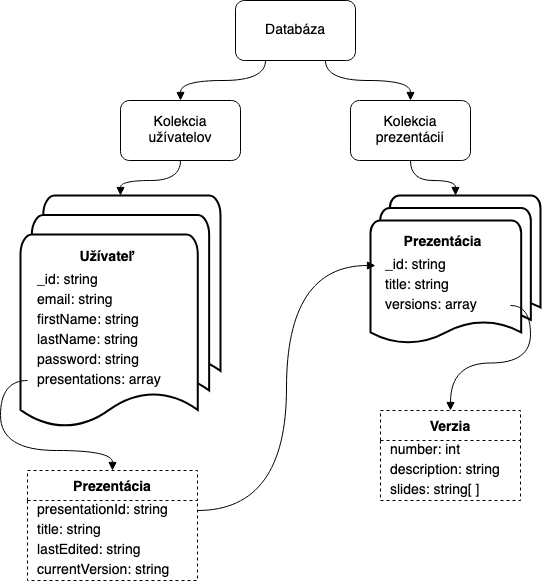
\includegraphics[scale=0.6]{obrazky/databaza.png}
        \caption{Znázornenie návrhu databáze.}
        \label{pic:database}
    \end{figure}
    
\section{Návrh backendu}
Serverová časť aplikácie prepojuje databázu s prezentačnou vrstvou. Obecne jej úkolom je sprostredkovanie komunikácie medzi nimi. Posiela HTTP odpovede na žiadosti klienta.

V tejto aplikácii má server za úlohu vytváranie, autentifikáciu, autorizáciu užívateľa, taktiež vytváranie, odstraňovanie, modifikovanie prezentácií a jeho verzií.

Návrh serverová čast sa skladá z troch hlavných vrstiev, ktoré medzi sebou komunikujú. Najnižšia je dátová vrstva ktorá má za úlohu vytváranie mongoose schém databáze a mapovanie modelov a entít. Najvyššia vrstva je vrstva API ktorá definuje koncové body a pristupuje k metódam repozitára. Tieto vrstvy sú prepojené vrstvou repozitára.

\subsection*{Vzor repozitára}
V aplikácii je implementovaný vzor repozitára. Tento vzor pomáha v odstránení redundantného kódu. Zapúzdruje základné \texttt{CRUD} metódy nad databázou. V aplikácii sa nachádzajú dva repozitáre, repozitár užívateľa a prezentácie. K metódam repozitára sa pristupuje z API vrstvy. 

\vspace{5mm}
\dirtree{%
.1 repository.
.2 presentationRepository.
.2 userRepository.
}
\vspace{5mm}

Repozitár užívateľa obsahuje následujúce metódy:
    \begin{itemize}
        \item\texttt{getUserById} - vyhľadávanie užívateľa podľa unikátneho identifikátora
        \item\texttt{getUserByEmail} - vyhľadávanie užívateľa podľa emailu
        \item\texttt{getUserToken} - získanie autentikačného tokenu užívateľa
        \item\texttt{saveNewUser} - uloženie nového užívateľa
        \item\texttt{newPresentationSummary} - vytvorenie nového stručného popisu prezentácie
        \item\texttt{updatePresentationSummary} - aktualizácia stručného popisu prezentácie
        \item\texttt{updatePresentationSummaryCurrentVersion} - aktualizácia aktívnej verzie prezentácie
        \item\texttt{deletePresentationSummary} - odstránenie stručného popisu prezentácie
    \end{itemize}
    
\vspace{5mm}
V repozitári prezentácie sa nachádzajú metódy: 
    \begin{itemize}
        \item\texttt{getPresentation} - získanie prezentácie podľa unikátneho identifikátora
        \item\texttt{newPresentation} - vytvorenie novej prezentácie
        \item\texttt{updatePresentation} - aktualizácia prezentácie
        \item\texttt{deletePresentation} - odstránenie prezentácie
        \item\texttt{deleteVersion} - odstránenie verzie prezentácie
    \end{itemize}
    
\subsection*{Vrstva API}
Vrstva API má za úlohu spracovávať dotazy od klienta na konkrétny koncový bod. Jednotlivé dotazy môžu obsahovať parametre v URI, takzvané query parametre, alebo parametre v tele dotazu. Pri úspešnom spracovaní dotazu API vráti HTTP odpoveď klientovi so správnym stavovým kódom \texttt{2xx}, kde čísla namiesto \texttt{x} sú doplnené podľa typu dotazu. Odpoveď môže obsahovať aj telo s obsahom. V aplikácii sa posiela obsah vo formáte JSON. Vrstva naďalej kontroluje či je dotaz správny, či je užívateľ prihlásený a má dostačujúce oprávnenie na vykonanie dotazu, alebo či požadované dáta existujú. Pri odchytení chyby API vráti chybovú hlášku so stavovým kódom \texttt{4xx} 

\begin{table}%[H]
    \centering
    \caption{Koncové body}
    \label{table:endpoints}
    \begin{tabular}{ |>{\centering\arraybackslash}m{18mm}|p{50mm}|p{70mm}|}
    \hline
    \textbf{GET} & \texttt{/api/user} & Získanie užívateľa  \\
    \hline
    \textbf{GET} & \texttt{/api/user/presentations} & Získanie prezentácií užívateľa  \\
    \hline
    \textbf{GET} & \texttt{/api/presentation} & Získanie konkrétnej prezentácie  \\
    \hline
    \textbf{POST} & \texttt{/api/auth/register} & Registrovanie užívateľa \\
    \hline
    \textbf{POST} & \texttt{/api/auth/login} & Prihlásenie užívateľa \\
    \hline
    \textbf{POST} & \texttt{/api/presentation} & Uloženie, alebo aktualizácia prezentácie  \\
    \hline
    \textbf{DELETE} & \texttt{/api/presentation} & Odstránenie prezentácie  \\
    \hline
    \textbf{DELETE} & \texttt{/api/presentation/version} & Odstránenie konkrétnej verzie prezentácie \\
    \hline
    \end{tabular}
\end{table}

    

\chapter{Implementácia}
Táto kapitola popisuje čitateľovi samotnú implementáciu aplikácie. Čitateľ sa oboznámi s použitými nástrojmi pri tvorení aplikácie a s postupom implementácie frontendovej a backendovej časti. Prvým bodom implementácie bolo vytvorenie zložky mono-repozitára zahrňujúci obe časti aplikácie.

\section{Git a GitHub}
Pred začatím písania zdrojového kódu sa najprv spojazdnil verzovací systém Git cez GitHub. Cieľom bolo verzovanie samotného zdrojového kódu aj dokumentácie. Pre jednoduchšiu orientáciu v repozitároch sa vytvorila GitHub organizácia, ktorá obsahuje monorepozitár pre zdrojový kód a repozitár pre dokumentáciu na jednom mieste. Monorepozitár je repozitár obsahujúci viacero projektov, v tomto prípade projekt klienta a servera. Organizácia aj repozitáre sú verejne dostupné pod odkazom:
    \begin{verbatim}
        https://github.com/AdamAbrahaamBC
    \end{verbatim}

GitHub ponúka projektom organizačnú tabuľku(project board). Tabuľka pomáha v organizovaní úloh a poskytuje jednoduchší prehľad projektu. Môže mať ľubovolný počet kolóniek, do ktorých sa prideľujú jednotlivé úlohy. V tomto projekte bolo postačujúce vytvorenie troch kolóniek. Kolónka \texttt{To Do} obsahuje ešte nezačaté úlohy, kolónka \texttt{In progress} úlohy, ktoré sa práve riešia a kolónka \texttt{Done} už dokončené a zatvorené úlohy. Pri vytvorení novej úlohy sa úloha automaticky priradí do kolónky \texttt{To Do}. Pri zvolení následujúcej úlohy musí byť manuálne premiestnená do kolónky \texttt{In Progress} a pri jej zatvorení sa automaticky premiestni do kolónky \texttt{Done}.


K jednotlivým úlohám sú pridelené štítky. Štítky označujú o aký typ úlohy sa jedná. Dostupné štítky projektu sú nasledujúce.

    \begin{itemize}
        \item\textbf{backend} - označuje úlohy týkajúce sa backendu
        \item\textbf{frontend} - označuje úlohy týkajúce sa frontendu
        \item\textbf{db} - označuje úlohy na databáze
        \item\textbf{bug} - označuje úlohy obsahujúce chybu v aplikácii
        \item\textbf{todo} - označuje zatiaľ nezačaté úlohy
        \item\textbf{done} - označuje dokončené úlohy
    \end{itemize}

\subsection{Implementácia frontendu}
Implementácia frontendu sa začala stiahnutím \texttt{Node.js}. Node.js obsahuje nástroj \texttt{npx} pre spúšťanie balíčkov. Pomocou npx sa vytvoril Nuxt.js projekt cez terminálový príkaz: \texttt{npx create-nuxt-app <názov-projektu>}. 

\vspace{5mm}
Po zadaní príkazu sa spustí sprievodca inštalácie, kde sa zvolil:
    \begin{itemize}
        \item správca balíčkov \texttt{npm}
        \item podpora pre \texttt{TypeScript}
        \item \texttt{Buefy} framework pre užívateľské prostredie
        \item komunikačný modul \texttt{axios}
        \item analyzačný nástroj zdrojového kódu \texttt{ESLint} 
        \item \texttt{jednostránkový} typ aplikácie(SPA)
    \end{itemize}
    
\vspace{5mm}
Balík Composition API je potrebné nainštalovať cez npm pomocou príkazu \texttt{npm install @nuxtjs/composition-api --save} a treba ho pridať medzi Nuxtom používané moduly v súbore \texttt{nuxt.config.js}.

Súbor \texttt{nuxt.config.ts} treba hneď na začiatku zvýrazniť. Je to súbor obsahujúci konfigurácie aplikácie. Nastavujú sa v ňom vlastnosti hlavičky aplikácie, ako názov, meta značky a ikonka. Obsahuje nastavenia smerovania, TypeScriptu, autentifikačného modulu, globálnych CSS súborov a ostatných rozširovacích modulov.

Nuxt.js udáva jednoduchý štartovací bod pre vývoj aplikácie. Po inicializácii projektu skonštruuje štruktúru aplikácie, ktorá je doplnená adresármi \texttt{composable} a \texttt{models}. štruktúru aplikácie dokopy tvoria nasledujúce adresáre:

\vspace{5mm}
\dirtree{%
.1 /client.
.2 /\.nuxt.
.2 /assets.
.2 /components.
.2 /composable.
.2 /dist.
.2 /layouts.
.2 /models.
.2 /node\_modules.
.2 /pages.
.2 /plugins.
.2 /store.
}
\vspace{5mm}

\subsection{Autentifikácia užívateľov}
Autentifikáciu užívateľov má na starosti autentifikačný nuxt modul. Modul sa nainštaloval cez npm, príkazom \texttt{npm install --save-exact @nuxtjs/auth-next} a pridal do nuxt konfiguračného súboru medzi moduly. Autentifikačný modul vyžaduje inštaláciu nuxt modulu \texttt{axios} pre HTTP komunikáciu. 

Middleware je globálne nastavený v nuxt konfiguračnom súbore na každú jednu trasu aplikácie okrem stránky prihlasovania, registrovania a zobrazenia prezentácie v prezentačnom móde. Na týchto stránkach je middleware manuálne vypnutý a sú dostupné bez autentifikácie. Neprihlásený užívateľ pri navštívení stránky, ktorá autentifikáciu vyžaduje je automaticky presmerovaný na prihlasovaciu stránku.

Modul funguje na báze schém. Schémy definujú logiku autentifikácie. Projekt môže obsahovať viacero schém pre rôzne typy prihlasovania, napríklad cez Facebook, Google, atď. V aplikácii je implementovaná lokálna schéma na báze JWT tokenov. Jej konfigurácia sa nachádza v konfiguračnom súbore. 

Modul poskytuje aplikačné rozhranie cez kľúčové slovo \$auth, ktoré je globálne dostupné cez kontext aplikácie. Prihlasuje sa cez funkciu \texttt{\$auth.loginWith('local', { data: PRIHLASOVACIE\_ÚDAJE })}. Modul pošle na prihlasovací koncový bod prihlasovacie údaje. Pri úspešnom prihlásení API vráti v HTTP odpovedi autentifikačný token užívateľa, ktorý sa uloží do koláčov(cookies) aplikácie a modul si automaticky vypýta údaje o užívateľovi podľa tokenu. Údaje užívateľa sú dostupné cez objekt \texttt{\$auth.user}. Odhlasuje sa cez \texttt{\$auth.logout()}.
\chapter{Testovanie}
\label{kapitola6}
V tejto kapitole sa nachádza popis a postup jednotlivých testov aplikácie, doplnený s obrázkami z testovacích prostredí. Pri testovaní sa použil nástroj Cypress a Postman. Práca s nimi je podrobnejšie popísaná nižšie.  

\section{Testovanie medzi dvomi stranami(End-to-End)}
Testovanie medzi dvomi stranami, alebo End-to-End testovanie slúži na testovanie funkcionality celej aplikácie. Narozdiel od jednotkových testov, ktoré testujú iba časť kódu, end-to-end testy prechádzajú celú aplikáciu z pohľadu užívateľa. Tieto testy sú dôležitou súčasťou aplikácie, umožňujú odchytenie chýb pri zmenách v zdrojovom kóde a zaručujú očakávané chovanie od začiatku až do konca.

\subsection{Cypress}
Cypress je nástroj pre webové aplikácie, ktorý umožňuje vytváranie testov medzi dvomi stranami. Nástroj ponúka širokú škálu funkcionalít pomocou ktorých sa dá otestovať každý jeden element webovej stránky. Cypress prechádza celú aplikáciu, simuluje správanie užívateľa. Umožňuje klikanie na tlačítka, písanie do políčok, alebo aj presmerovanie na inú URL adresu. Poskytuje prehľadné užívateľské rozhranie kde simuluje užívateľom vybraný prehliadač. Jednotlivé testy sa dajú spustiť naraz, ale aj zvlášť po častiach. Po vytvorení účtu a prihlásení, cypress uchováva históriu testov, ku ktorým sa dá hocikedy vrátiť. Nástroj umožňuje náhľad do testu v priebehu testovania, kde je vidieť každý jeden krok testu, s ktorými elementami sa pracovalo a aké akcie sa vykonali. K jednotlivým krokom sa v ktoromkoľvek okamihu počas testovania dá vrátiť.

Cypress sa inštaluje klasicky ako každý iný balík cez správcu balíčkov npm a spúšťa sa cez príkaz v termináli \texttt{npx cypress open}. Po prvom spustení sa v hlavnom adresári klienta vytvorí zložka \texttt{cypress}, s ktorou sa ďalej pracuje. Jednotlivé testy sa nachádzajú v zložke \texttt{cypress/integration}. End-to-End testy v aplikácii sú rozdelené na dve hlavné časti, \texttt{auth} a \texttt{presentation}. K jednotlivým elementom používaným v testoch sa pristupuje cez HTML data atribút. Tieto elementy sú v šablóne označené cez atribút \texttt{data-test}, napríklad: \texttt{<b-input data-test="email" />}. Pri ich potrebe sa element vyhľadá a zvolí pomocou cypress funkcie a vykoná sa potrebná akcia nad nim.

Po úspešnom priebehu, cypress označí test zelenou fajkou a pri narazení na chybu červeným krížom. Po dokončení testovanie sa zobrazí súhrn testovania a čas v sekundách trvania celého testu viz. obrázok \ref{pic:cypress}.

    \begin{figure}[!hbt]
        \centering
        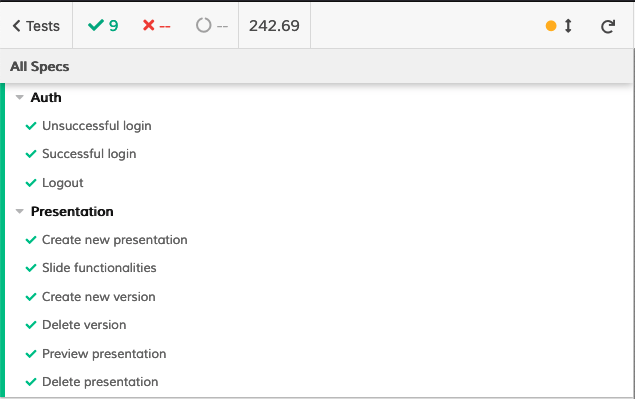
\includegraphics[scale=0.4]{obrazky/cypress.png}
        \caption{Súhrn dokončeného testovania}
        \label{pic:cypress}
    \end{figure}

\subsection*{Autentifikačné testy}
Autentifikačné testy sa nachádzajú v súbore \texttt{cypress/integration/auth.ts}. Tento súbor obsahuje testy:

    \begin{itemize}
        \item\textbf{Unsuccessful Login} - testuje sa zobrazenie chybovej hlášky pri neúspešnom prihlásení cez tlačítko.    
        \item\textbf{Successful Login} - testuje sa vyplnenie správnych prihlasovacích údajov a prihlásenie cez tlačítko.
        \item\textbf{Logout} - testuje sa odhlásenie cez tlačítko a presmerovanie na stránku prihlásenia.
    \end{itemize}
    
\subsection*{Testy prezentácie}
V súbore \texttt{cypress/integration/presentation.ts} sa nachádzajú všetky testy týkajúce sa prezentácií, od ich tvorby až k odstráneniu. Tento súbor obsahuje testy:

    \begin{itemize}
        \item\textbf{Create new presentation} - v tomto teste sa kontroluje, že daný užívateľ najprv nemá žiadne vytvorené prezentácie. Prezentácia sa vytvorí cez tlačítko. \texttt{CREATE NEW} a otestuje sa, či URL adresa odpovedá adrese \texttt{/presentation/new} a či je editor viditeľný. Cez tlačítko sa otvorí panel pre uloženie prezentácie a následne sa vyplnia potrebné údaje pre uloženie. Pomocou tlačítka sa vráti na domovskú stránku, kde sa skontroluje či zoznam obsahuje uloženú prezentáciu.
        
        \item\textbf{Slide functionalities} - v tomto teste sa kontrolujú všetko funkcionality nad stránkami prezentácie. Najprv sa otvorí prezentácia v editore cez tlačítko na domovskej stránke. Cez tlačítko sa otvorí bočný panel obsahujúci stránky prezentácie. Prezentácia v tomto okamihu obsahuje iba jednu stránku. Otestuje sa, že pri jednej stránke je tlačítko odstránenia stránky nefunkčné. Nasleduje test kopírovania a vloženia stránky. Otestuje sa pridanie novej stránky cez tlačítko a jeho odstránenie. V poslednom kroku sa kontroluje mriežkový pohľad stránok.
        
        \item\textbf{Create new version} - v tomto teste sa pracuje s verziami prezentácie. Znova sa prezentácia otvorí v editore, kde sa uloží pod iným názvom ako verzia číslo 2. Na domovskej stránke sa otestuje, že zoznam stále obsahuje iba jednu prezentáciu, ale s iným názvom. Zobrazí sa detail prezentácie a skontroluje sa počet prezentácií. Otestujú sa rôzne popisy jednotlivých verzií. Otvorí sa verzia číslo 2 v editore a uloží sa pod iným názvom a rozličným popisom pod rovnakou verziou. Na domovskej stránke sa znova skontroluje počet prezentácií, počet verzií a či verzia číslo 2 obsahuje nové údaje. 
        
        \item\textbf{Delete version} - v tomto teste sa rieši odstránenie verzie prezentácie. Mazanie sa uskutoční cez tlačítko na domovskej stránke, aplikácia si vyžiada potvrdenie o mazaní. Po odstránení sa skontroluje počet verzií prezentácie.
        
        \item\textbf{Preview presentation} - v tomto teste sa testuje zobrazenie prezentácie v prezentačnom móde cez tlačítko na domovskej stránke. Kontroluje sa či URL adresa obsahuje text \texttt{/preview}.
        
        \item\textbf{Delete presentation} - test kontroluje úspešné odstránenie celej prezentácie cez tlačítko na domovskej stránke. Po odstránení sa testuje prázdny zoznam prezentácií. 
    \end{itemize}
    
\section{Testovanie aplikačného rozhrania}
Aplikačné rozhranie sa počas vývoja testovalo cez nástroj Postman. Postman je pomôcka, ktorá umožňuje zasielanie HTTP dotazov na koncové body a prijímanie odpovedí od nich. Nástroj poskytuje prehľadné užívateľské rozhranie, kde stačí zadať URL adresu koncového bodu. Užívateľské rozhranie obsahuje históriu poslaných dotazuv, ku ktorým sa dá kedykoľvek vrátiť. Postman taktiež umožňuj jednoduché pridávanie query parametrov, obsahu tela dotazu a upravovanie hlavičky dotazu. Odpoveď na dotaz je možné zobraziť vo viacerých formátoch. Prostredie nástroja je zobrazené na obrázku \ref{pic:postman}.

    \begin{figure}[!hbt]
        \centering
        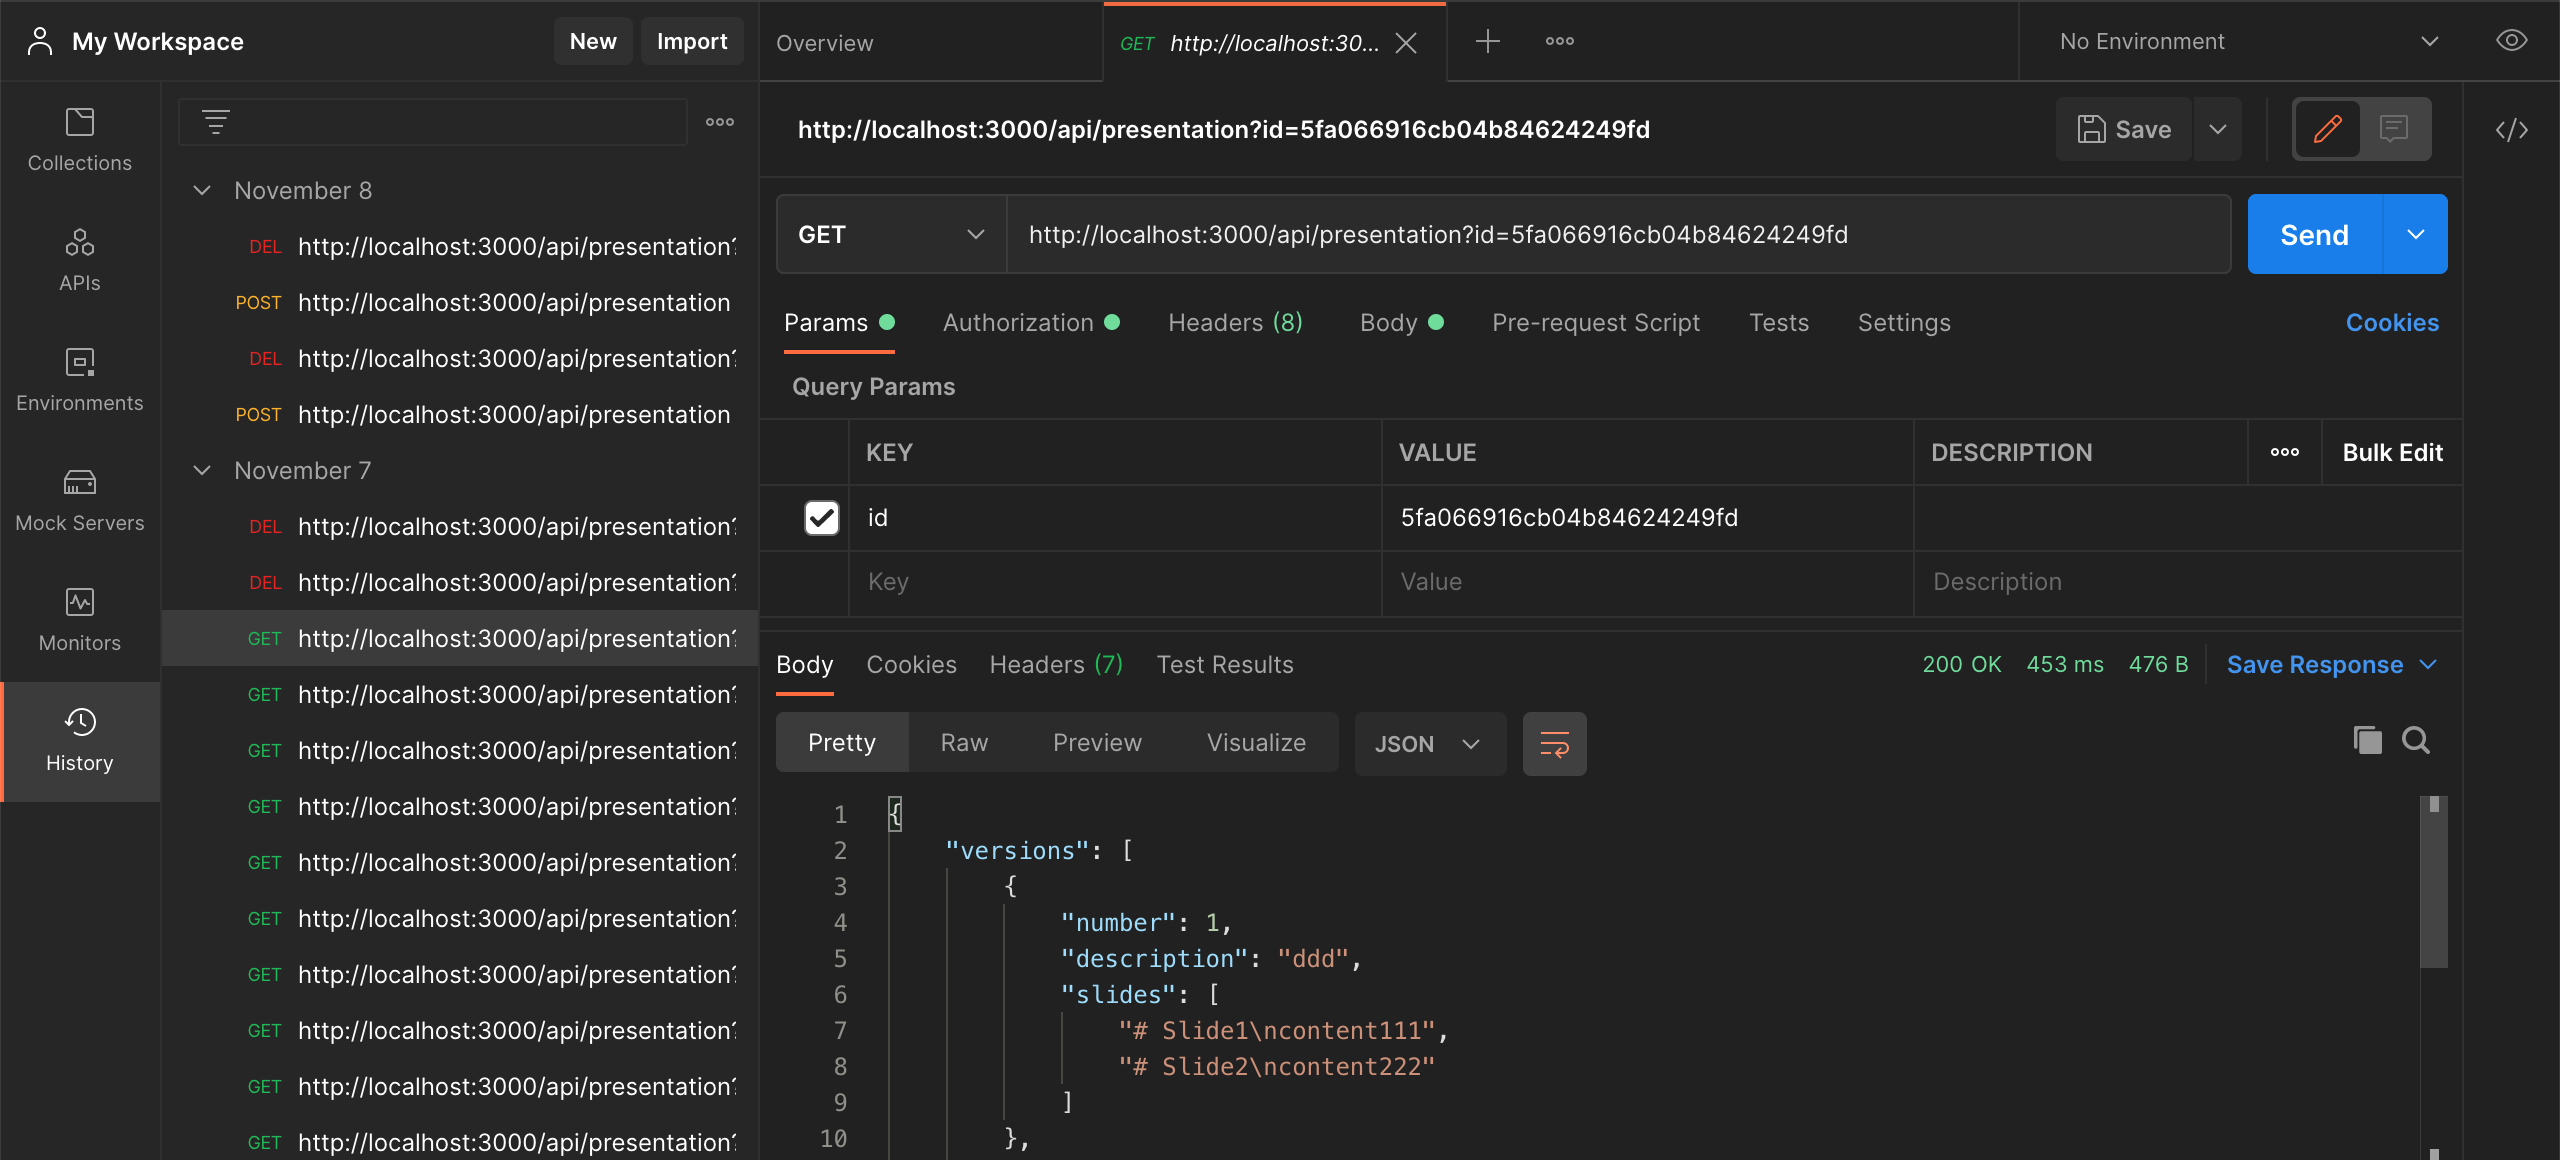
\includegraphics[scale=0.3]{obrazky/postman.png}
        \caption{Prostredie nástroja Postman}
        \label{pic:postman}
    \end{figure}
  
  % Kompilace po částech (viz výše, nutno odkomentovat)
  % Compilation piecewise (see above, it is necessary to uncomment it)
  %\subfile{projekt-01-uvod-introduction}
  % ...
  %\subfile{chapters/projekt-05-conclusion}


  % Pouzita literatura / Bibliography
  % ----------------------------------------------
\ifslovak
  \makeatletter
  \def\@openbib@code{\addcontentsline{toc}{chapter}{Literatúra}}
  \makeatother
  \bibliographystyle{bib-styles/Pysny/skplain}
\else
  \ifczech
    \makeatletter
    \def\@openbib@code{\addcontentsline{toc}{chapter}{Literatura}}
    \makeatother
    \bibliographystyle{bib-styles/Pysny/czplain}
  \else 
    \makeatletter
    \def\@openbib@code{\addcontentsline{toc}{chapter}{Bibliography}}
    \makeatother
    \bibliographystyle{bib-styles/Pysny/enplain}
  %  \bibliographystyle{alpha}
  \fi
\fi
  \begin{flushleft}
  \bibliography{literatura}
  \end{flushleft}

  % vynechani stranky v oboustrannem rezimu
  % Skip the page in the two-sided mode
  \iftwoside
    \cleardoublepage
  \fi

  % Prilohy / Appendices
  % ---------------------------------------------
  \appendix
\ifczech
  \renewcommand{\appendixpagename}{Přílohy}
  \renewcommand{\appendixtocname}{Přílohy}
  \renewcommand{\appendixname}{Příloha}
\fi
\ifslovak
  \renewcommand{\appendixpagename}{Prílohy}
  \renewcommand{\appendixtocname}{Prílohy}
  \renewcommand{\appendixname}{Príloha}
\fi
%  \appendixpage

% vynechani stranky v oboustrannem rezimu
% Skip the page in the two-sided mode
%\iftwoside
%  \cleardoublepage
%\fi
  
\ifslovak
%  \section*{Zoznam príloh}
%  \addcontentsline{toc}{section}{Zoznam príloh}
\else
  \ifczech
%    \section*{Seznam příloh}
%    \addcontentsline{toc}{section}{Seznam příloh}
  \else
%    \section*{List of Appendices}
%    \addcontentsline{toc}{section}{List of Appendices}
  \fi
\fi
  \startcontents[chapters]
  \setlength{\parskip}{0pt} 
  % seznam příloh / list of appendices
  % \printcontents[chapters]{l}{0}{\setcounter{tocdepth}{2}}
  
  \ifODSAZ
    \setlength{\parskip}{0.5\bigskipamount}
  \else
    \setlength{\parskip}{0pt}
  \fi
  
  % vynechani stranky v oboustrannem rezimu
  \iftwoside
    \cleardoublepage
  \fi
  
  % Přílohy / Appendices
  \ifenglish
    \input{projekt-30-prilohy-appendices-en}
  \else
    \input{projekt-30-prilohy-appendices}
  \fi
  
  % Kompilace po částech (viz výše, nutno odkomentovat)
  % Compilation piecewise (see above, it is necessary to uncomment it)
  %\subfile{projekt-30-prilohy-appendices}
  
\end{document}
